 \documentclass[conference]{IEEEtran}
\usepackage{subfig}
\usepackage{wrapfig}
 \usepackage{amsmath}
 \usepackage{url}
 \usepackage{pifont}
 \usepackage{times}
\usepackage{rotating}
%\usepackage{balance} 
\usepackage{color, colortbl}
\usepackage{graphicx}
\usepackage{algorithmicx}
\usepackage{program}
\usepackage{cite}
\usepackage{alltt}
\newcommand{\eq}[1]{Equation~\ref{eq:#1}}
\newcommand{\bi}{\begin{itemize}}
\newcommand{\ei}{\end{itemize}}
\newcommand{\be}{\begin{enumerate}}
\newcommand{\ee}{\end{enumerate}}
\newcommand{\tion}[1]{\textsection\ref{sec:#1}}
\newcommand{\fig}[1]{Figure~\ref{fig:#1}}
\definecolor{lightgray}{gray}{0.975}
\usepackage{fancyvrb}
\usepackage{stfloats}
\usepackage{multirow}
\usepackage{listings}
\usepackage{amsmath} 
\DeclareMathOperator*{\argmin}{arg\,min} 
\DeclareMathOperator*{\argmax}{arg\,max} 


\definecolor{darkgreen}{rgb}{0,0.3,0}

\usepackage[table]{xcolor}
\definecolor{Gray}{rgb}{0.88,1,1}
\definecolor{Gray}{gray}{0.85}
\definecolor{Blue}{RGB}{0,29,193}
\newcommand{\G}{\cellcolor{green}}
\newcommand{\Y}{\cellcolor{yellow}}


\definecolor{MyDarkBlue}{rgb}{0,0.08,0.45} 
\newenvironment{changed}{\par\color{MyDarkBlue}}{\par}

\newcommand{\ADD}[1]{\textcolor{MyDarkBlue}{{\bf #1}}}
\newcommand{\addit}[1]{\begin{changed}\input{#1}\end{changed}}

\usepackage{color}
\usepackage{listings}
\usepackage{setspace}

\definecolor{Gray}{gray}{0.9}
\newcommand{\kw}[1]{\textit{#1}}
\newcommand{\quart}[4]{\begin{picture}(75,6)
  {\color{black}\put(#3,3){\circle*{2.5}}\put(#1,3){\line(1,0){#2}}}\end{picture}}
% New Commands

\definecolor{Code}{rgb}{0,0,0}
\definecolor{Decorators}{rgb}{0.5,0.5,0.5}
\definecolor{Numbers}{rgb}{0.5,0,0}
\definecolor{MatchingBrackets}{rgb}{0.25,0.5,0.5}
\definecolor{Keywords}{rgb}{0,0,1}
\definecolor{self}{rgb}{0,0,0}
\definecolor{Strings}{rgb}{0,0.63,0}
\definecolor{Comments}{rgb}{0,0.63,1}
\definecolor{Backquotes}{rgb}{0,0,0}
\definecolor{Classname}{rgb}{0,0,0}
\definecolor{FunctionName}{rgb}{0,0,0}
\definecolor{Operators}{rgb}{0,0,0}
\definecolor{Background}{rgb}{1,1,1}

\lstnewenvironment{python}[1][]{
\lstset{
mathescape,
numbers=#1,
numberstyle=\footnotesize,
numbersep=0.5em,
xleftmargin=0em,
framextopmargin=2em,
framexbottommargin=2em,
showspaces=false,
showtabs=false,
showstringspaces=false,
tabsize=2,
% Basic
basicstyle=\ttfamily\small\setstretch{0.8},
backgroundcolor=\color{Background},
language=Python,
% Comments
commentstyle=\color{Comments}\slshape,
% Strings
stringstyle=\color{Strings},
morecomment=[s][\color{Strings}]{"""}{"""},
morecomment=[s][\color{Strings}]{'''}{'''},
% keywords
morekeywords={[1]import,from,class,def,for,while,if,is,in,elif,else,not,and,or,print,break,continue,return,True,False,None,access,as,,del,except,exec,finally,global,import,lambda,pass,print,raise,try,assert, dot, norm, zip, sorted},
keywordstyle={[1]\color{Code}\bfseries},
% additional keywords
morekeywords={[3]fastmap, project, furthest, split, WHERE,clusterer, getContours, envied, fWeight, nearestContour, projection, mutate, HERE, knn},
keywordstyle={[3]\color{Keywords}\bfseries},
morekeywords={[2]@invari},
keywordstyle={[2]\color{Decorators}\slshape},
emph={self},
emphstyle={\color{self}\slshape},
%
}}{}
 
\title{Learning Actionable Analytics 
 (with applications for reducing defects and reducing runtimes)}
\author{
% You can go ahead and credit any number of authors here,
% e.g. one 'row of three' or two rows (consisting of one row of three
% and a second row of one, two or three).
%
% The command \alignauthor (no curly braces needed) should
% precede each author name, affiliation/snail-mail address and
% e-mail address. Additionally, tag each line of
% affiliation/address with \affaddr, and tag the
% e-mail address with \email.
%
% 1st. author
Rahul Krishna, Tim Menzies, Xipeng Shen\\
       \affaddr{Computer Science, NcState, USA}\\
       \{i.m.ralk, tim.menzies, xipengshen\}@gmail.com
% 3rd. author
 % use '\and' if you need 'another row' of author names
% 4th. author
\and
 Andrian Marcus\\
       \affaddr{Computer Science, UtDallas, USA}\\
       {amarcus@utdallas.edu} }


  \pagestyle{plain}
\begin{document}
  \maketitle
  
  % make the title area
  
   
  \begin{abstract}
 As business users demand more insightful
 analytics, data scientists need to change
 their tools. Instead of merely predicting 
 some result, they also need tools that generate ``policy advice'';
 i.e. suggestions on  how to change values in order to
 improve on some predicted value.
 
 This paper proposes one such policy
 generator. ``HOW'' is a near-linear-time
 tool for proposing changes to independent
 variables in order to improve on 
 the predictions of the dependent variables. Unlike other approaches
 for learning optimizations to software does not require
 an underlying of the domain (rather, HOW automatically
 learns that model as part of its operation). 
 
 This paper uses  HOW to learn methods
 to reduce defects and decrease program runtime.
 For the test data of this paper, the improvements generated by HERE can reduce
 defect counts as well as runtimes by up to
 50\% of their original values.
  \end{abstract}
  \begin{IEEEkeywords}
Instance-based reasoning, defect prediction, random forest, optimization.
  \end{IEEEkeywords}
  
\section{Introduction}
Business  users are now demanding that data mining tools
be augmented with tools to support  business-level
interpretation of that data. For example,
at a  panel on software analytics at ICSE'12,
industrial practitioners lamented the state of the art in data mining
and software engineering~\cite{menzies12a}. Panelists commented that
``prediction is all well and good, but what about decision
making?''. That is, these panelists are more interested in the interpretations
that follow the mining, rather than just  the mining. For example:
\bi
\item Instead of just accepting  {\em predictions} on how many 
 software defects
to expect,  business users might now demand a {\em plan} to
reduce the likelihood of those defects;
\item Instead of just accepting {\em predictions} on the runtime
time of their software, business users might now demand
a {\em plan} to reduce that runtime.
\ei
In these two points, we say that a ``plan'' is a  set of proposed changes in order to better achieve some goal. 
Generating {\em plans} is a  very different task the standard
data mining tasks of {\em predicting} some discrete or numeric class.
Predictors
and classifiers only tell us what {\em is} while planners 
  tell us {\em what to change}. For the kind of business user
discussed above, planners are the preferred to mere prediction systems
since, as one gruff user once shouted at us:
\begin{quote}
{\em ``Don't tell me what \underline{is};
tell me what to \underline{change}.''}
\end{quote}
In order to satisfy the demands of this new kind of business user, we  study the generation of {\em plans} in the context
of software analytics.  
This paper presents
HOW, a novel  {\em instance-based planner} that runs in near-linear time.
In the experiments shown below, we see that HOW's plans can
significantly reduce the expected
value of:
\bi
\item Software defects in certain object-oriented JAVA systems listed in \tion{oo}:  Ant Camel, Ivy, Jedit, JBeans, Log4, Lucene, Poi, Synapse, Velocity, Xalan, Xerces;
\item The runtime of the software systems discussed in \tion{cpu}: Berkeley DB, Apache, SQLite, LLVM, 
  x264.
\ei
HOW's instance-based reasoning  makes its conclusions by
studying the space of examples. This is a very different approach to
{\em model-based planners} that use the model
as sub-routine within a Monte Carlo simulation~\cite{me07f} or the evolutionary 
programming methods explored by the search-based software
engineering community~\cite{krall14,harman12dec}. 
We find   HOW's instance-based approach useful since it can be applied
to domains that lack a model, but possess a historical log of observed behaviours.

Instance-based reasoning is also useful if building and certifying a model   takes a long time. Such slow-to-build models exist in software engineering. For  example, in previous work~\cite{me07f} we used models
developed by Boehm's group at the University of Southern California.
Some of those models took decades to develop and mature (from 1981~\cite{boehm81} to 2000~\cite{boehm00b}).  This is not an isolated example. One of us (Menzies) teaches a graduate class in automated model-based software engineering. 
Students in that class are asked to find (or build) a non-trivial model of
some software process (where ``non-trivial'' means something that processes
a  model at least an order of magnitude more complex than Brooks' Law). 
While the  number of such models has been growing in recent years\footnote{See the
catalogue at goo.gl/nv2AVK.}, 
the total number remains very small-- which is an observation consistent with
SE models typically require  much effort to build and certify.

Finally, even when there is an existing model, instance-based reasoning can be useful.
Sometimes  it is easier to access instances of a model's behaviour than the model
itself. For example, in prior work with Martin  Feather from the Jet Propulsion 
Laboratory~\cite{fea02a},  our research partner could not share a
propriety model from within the NASA firewalls. However, they could share 
logs of the input/output of that model.
 
In summary, this paper makes five contributions:
\be
\item A general framework for augmenting a prediction system such that
it becomes a planning system;
\item A  test that recognizes  when we should {\em not}  plan: in summary, our kind of planning is
not recommended in domains that  generate poorly performing predictors;
\item A general verification rig for assessing the value of plans generated within this rig.
\item The HOW  instance-based planner.
\item A proof that HOW runs in near-linear time.
\item An experimental validation that the HOW planner is useful for reducing the
expected values of software defects and software runtimes (at least, for the data sets studied here).
\ee
The rest of this paper is structured as follows.

 

\section{From ``Prediction'' to ``Planning''}
A major  problem with building a planning mechanism in software engineering is ``how to verify the generated
plans?''. For example,  in the experiments shown below,  HOW comments  on how to reduce
software defects by adjusting certain static code parameters of the code\footnote{Such parameters can be automatically adjusted using code refactoring
tools, as shown by Binkely et al. in 2006~\cite{Binkley2006} and more recently by Mkaouer et al. in 2015~\cite{Mkaouer15}.}. How are we to verify that HOW's recommendations actually work? 

Some organizations have the resources to 
run repeated trials to assess the effect of different treatments.
For example, in one remarkable recent study, Bente et al. report results
were the same specification was developed into a product by four different organizations~\cite{Anda2009}. Given those kind of resources, it would be possible
to (say) take a code base, assign it to $N$ different teams, apply
HOW's plans the code used by  $N/2$ teams, then check in 12 months time
if those halves of the teams have fewer defects than the other.  

Very few industrial or research groups have access
to the kinds of resources using by Bente et al. (evidence: in the size years since the
publication of that work, we know of only one of two similar studies). Hence, it
we wish to verify HOW's plans, then some other approach is required that is less
resource intensive.

\subsection{Proposed Framework}

We propose using prediction systems (built by data mining) as a verification
tool for planners. In domains with data, from which data miners can build
predictors of adequate performance, then those predictors can assess the value
of the changes proposed by HOW.
As shown in \fig{work}, 
project data is divided into two disjoint sets {\em train} and {\em test}
(so {\em train} $\cup$ {\em test} $=\;\emptyset$).
Next, from the train set, we build both a {\em planner} as well
as a {\em predictor}. Our general framework does not   commit to any particular  choice
of {\em planner} or {\em predictor}. For the purposes of this discussion 
our {\em planner}
will be HOW (discussed below)and our
our {\em predictors} will be the Random Forest and Random Forest
Regressor\footnote{Decision tree learners find the attribute whose value's
select for for sections of the data with least variation in the class
variable. Decision tree learners then recurse on each selection~\cite{breiman84}. A random forest is a set of decision trees, each built
from some random subset of the rows and columns. The conclusions
of the forest are a ``vote'' generated by all the trees~\cite{Breiman2001}. 
A standard Random Forest predicts for a discrete class variable while
a Random Forest Regressor generates numeric predictions.} taken from the SciKit
Learn toolkit~\cite{Pedregosa2012}.

Turning now to the {\em test} data, this is based to the {\em predictor}
to generate a baseline {\em before} performance score.
Note that if our {\em predictors} fail to perform adequately on the test data,
then we cannot trust them to comment on our plans. Accordingly,
if that performance is unsatisfactory, we abort.
Else, we (1)~apply the {\em planner} to alter the {\em test} data;
then (2)~apply the {\em predictor} to the altered data {\em test'};
then (3)~return the performance delta.

\subsection{When Not to Plan: Problem of Poor Planner}

The clear advantage of this approach is that it can be readily and automatically
applied to domains with historical data. That said, the drawback with this approach
is that our assessment of the plans is only as good as the predictor. To 
mitigate for this {\em problem of poor planners}, it is wise to demand high standards form the {\em
satisfactory} threshold used in this \fig{work}. 



\begin{figure}[!t]
\small
\[  
\begin{array}{r}
project\\
data
\end{array} 
\left\{\begin{array}{l}\mathit{train}
        \left\{\begin{array}{l}
                \mathrm{learn\;a\;}\mathrm{predictor\;}\mathrm{e.g.\;Random\;Forest}\\
                \mathrm{learn\;a\;}\mathrm{planner\;}\mathrm{e.g.\; HOW}
              \end{array}\right.
       \\
      ~\\
\mathit{test}  
    \left\{\begin{array}{l@{~}l}
           \mathit{before}& =\mathrm{predictor}(\mathit{test})\\
           \mathrm{\bf if\;}\mathit{before} & <  \mathit{satisfactory}\\
           \mathrm{\bf then}  & \mathrm{{\bf return}\; 0}\\~\\
           \mathrm{\bf else} &
           \left\{
            \begin{array}{l}
                \mathit{test'} = \mathrm{planner}(\mathit{test})\\
                \mathit{after} =\mathrm{predictor}(\mathit{test'})\\ 
                \mathrm{{\bf return}\;} \mathit{after} /  \mathit{before}
            \end{array}
          \right.
   \end{array}\right.
\end{array} \right. 
\] 
 
\caption{How to use {\em predictors} for {\em planning}.}\label{fig:work}
\end{figure}

How prevalent is the problem of poor planners? While
this is hard to answer in the general case, we can say that for the 17 data
sets explored in this study, only 3 suffer from this problem.
This study's    data   from two  types of domains:
\bi
\item
In one type, we 
build plans to change static code attributes in order to reduce defects in
Java classes.  Here,,
performance can be measured in terms of recall (percent of faulty classes in
the test data detected
by the {\em predictor}). Using engineering judgement, we define satisfactory recall as anything over   70\%. 
\item 
In the other type, we   build
plans to change configurations settings within a Makefile such that the resulting compiled
code will run faster. Here, performance can be measured in terms of difference
between the predicted runtime $p$ of test case items and their actual runtimes $a$
using  $s= 1- \frac{abs(a - p)}{a}$.
Using engineering judgement, we define satisfactory $s$ as anything over   70\%. 
\ei
This paper explores 12 static code data sets
Ant, Camel, Ivy, Jedit, JBeans, Log4, Lucene, Poi, Synapse, Velocity, Xalan, Xerces\footnote{Available from the object-oriented defects section of the PROMISE respository openscience.us/repo/defect/ck.} and five configuration data sets Berkeley DB, Apache, SQLite, LLVM,
  x264\footnote{Available from the performance prediction section of PROMISE
  http://openscience.us/repo/performance-predict.}. For each of these data sets,
  we generated 25 {\em before} scores from
  random split train:test splits in the ratio 4:1 train.
 The median {\em before} scores from  the static code data sets were:
%issue24
\[\mathrm{recall}=\{98,88,86,84,82,81,79,78,78,\overbrace{55,23,20}^{\mathrm{JBeans,Poi,Xalan}}\}\]
The median {\em before}   scores from  the configuration data were:
%issue 24
\[s=\{98,97,95,88,92\}\]
Note that we need to abort planning in only $3/17$ of our data sets.  
 
\subsection{Are These Plans ``Causal''?}
With one small variation,  the above framework can be used to check if the learned
plans can be said to {\em cause} a change in the domain being explored.

In the literature, there are two main definitions of causality: Hill's H-causality~\cite{Hill1965}
and Granger's G-casualty~\cite{granger80}. 
Of the two, Hill's definition is the most strict. An effect
is H-causal if it satisfies nine criteria including:
\be
\item
Plausibility;
\item
Strength of the effect; 
\item
Specificity: locality of the effect
to specialized groups;
\item
Support by experimental evidence;
\item
Coherence between cause-effects noted
in the field and in laboratory samples;
\item
Temporally: the effect has to follow the cause;
\item
Analogy: similar causes have similar effects;
\item
Biological gradient: more exposure to the cause leads to more of an
effect)
\item
Consistency: the same cause-effect pairings have been seen by different persons
in different places.
\ee
It is hard to demonstrate H-causality in software engineering.
For example, Hill's criteria emphasises repeatability and laboratory studies-- both of which are
hard to perform in software engineering (e.g. see the continued debate about
the value of using undergraduate students to surrogates for industrial
practitioners in software engineering research~\cite{Carver2003}). Also, Hill's requirement
for consistency is far easier to achieve in studies of small closed systems (e.g. bacteria in a petri dish)
than in large socio-technical systems (e.g. open source projects). 

The practical difficulties associated with Hill's criteria lead Granger~\cite{granger80}
to propose another criteria\footnote{Granger  notes that
his proposal was based on earlier work by Norbert Weiner~\cite{Seth2007}.}.
G-causality is based on building predictions based on {\em past} data,
then showing that this works for {\em future} data~\cite{granger80}. 

Note that the standard 10-way cross-validation
procedure  in data mining does {\em not} demonstrate G-causality.  In a N-way cross-val experiments, the data is divided into $N$ bins.  
$N-1$ bins are used for learning and the results are tested
on the  remaining bin.
Cross-validation is then repeated $N$ times, each time using a different bin for the test set.
This approach can not be used to demonstrate causality since, if the initial data is collected
over (say) $N$ months, then it is possible that the test set contains observations collected
{\em before}   items seen in the training set. 

Jiang et al.~\cite{me11f} and Lumpe et al.~\cite{me11f} propose a modification to cross-validation which lets them
demonstate G-causal defect effects in softwrare engineering.
They divide project data  into $N$ bins, each of with contain data collected at similar times.
They then sort those bins (on the collection date) and use bins $i,j$ to predict for $k$ where 
$i<j<k$. 

We adapt the work of Jiang,Lumpe et al.  as follows. In  \fig{work}, we demand that the {\em test}
data is not collected before the {\em train} data.  With that change,
we can reasonably claim that the plan's generating by HOW are G-causal.

\section{Releated Work}

Our prior work in generating policies relied upon a Monte Carlo
analysis of an underlying model~\cite{me07f}. This approach had three major problems.
Firstly, enough domain knowledge had to be collected to build that model
and this can take a long time. For example, in our previous work we used three software process models from
the Unviersity of Southern California that were initially
developed and updated for nearly two decades from 1981~\cite{boehm81} to 2000~\cite{boehm00b}.

Secondly, there is the computational cost of running those models.
While 

~\cite{}-- which suffered from the problem of (a)~the effort required to collect the domain knowledge to build
problem in certifying the underlying model;
 (b)~the computational problem of running that model enough
times to learn patterns in that data; and (c)~ requrearea used large scale simulations or large


While
our case studies are defect and runtime reduction, HERE is a general
purpose algorithm that could be applied to any table of data with at least
one column whose values can be sorted from ``desired'' to ``undesired''.

\section{Related Work}
Policy generation is different to standard data mining in that the 
latter is most concerned with what {\em is} rather than {\em what to do}.
For example, a classification or prediction system such as C4.5~\cite{quinlan92} or CART~\cite{breiman84} can predict for a discrete or continuous class variable
(respectively). As such, they can be used as a sub-routine within a
policy generator. For example, later in this paper we will use the CART
prediction system to assess the policies generated by HERE.


Policy generation with HERE is different to the recommendor systems.
As described by Robillard and Walker~\cite{rob14}, recommendor systems
in software engineering
are less {\em directive} and more    {\em collaborative} than policy
generators:
\bi
\item
Directive systems such as HERE tell developers exactly what to do
(e.g. ``use these settings in a Makefile'') 
\item
Collaborative systems are more suggestive guides that
help (e.g.) programmers focus on very small sets
with  very large libraries of code of documentation.
\ei
Collaborative systems may not presume to know what to do
in that smaller set (while the directive systems would issue an edict
such as  ``change this to that'').

We also distinguish HERE's policy generation fro the multi-objective optimization methods explored by Harman and Krall and Menzies and 
and many others.



Previous with have explored model-based policy generation with STAR,
NOVA, and instance-based policy generation with  W2.

refactoring XXX

Finally, we note that HERE is a temporal transfer learner.


{\bf RQ1: Can Instance-based Learning techniques be used to create Planning tools that can better analyse software defect?} 


{\bf RQ2: Can lessons learnt from local policy generators be useful for generating solutions that can be used to mitigate defects in software systems?} 

{\bf RQ3: Can such instance-based planners be applied to other software engineering paradigms?}
We check if the proposed instance-based planner is applicable to performance prediction.

\section{Motivating Example}
\section{Background}
\section{Instance Based Learning}

Assessing the quality of solutions to a real-world problem can be extremely hard~\cite{menzies2005xomo}. In several software engineering applications, researchers have models that can emulate the problem, for instance there is the COCOMO effort model~\cite[p29-57]{boehm2009software}, the COQUALMO defect model~\cite[p254-268]{boehm2009software}, Madachy’s schedule risk model~\cite[p284-291]{boehm2009software}, to name a few. Using these models it is possible to examine several scenarios in a short period of time, and this can be done in a reproducible manner. However, models aren't always the solution, as we shall see. 

There exist several problems where models are hard to obtain, or the input and output are related by complex connections that simply cannot be modeled in a reliable manner, or generation of reliable models take prohibitively long ~\cite{Ludewig2003}. Software defect prediction is an excellent example of such a case. Models that incorporate all the intricate issues that may lead defects in a product is extremely hard to come by. Moreover, it has been shown that models for different regions within the same data can have very different properties \cite{localvsglobal}. This makes it extremely hard for one to design planning systems that are capable of mitigating these defects.

An alternative approach would be to make use of an instance based approach, an example of case based reasoning strategy, in place of the conventional model based approach. Instance based approaches have been used extensively by the effort estimation community, see~\cite{keung2008analogy, 6600685, walkerden1999empirical, shepperd1997estimating, kocaguneli2010use}. 

This approach has been proposed as an alternative to closed form mathematical models or other modeling methods such as regression \cite{keung2008analogy}. There are several other reasons for instance based approaches being a useful tool, see~\cite{6600685}. As pointed out by~\cite{walkerden1999empirical} it can be used with partial knowledge of the target project at an early stage which could be a very useful tool in preventing software defects. Instance based approaches are also rather robust in handling cases with sparse samples \cite{1438374}. All these features are desirable and suggest that instance-based approach is a useful adjunct to traditional model based approach. 

In this paper the instance based learning principle is used to first cluster the training data and then create contours in the data. These contours can then be used by test cases to infer meaningful information in order to improve it. The entire process is described in greater detail in the following sections. We would like to stress that the purpose of our work is not to promote instance-based planning over model based analytics, rather it is to suggest an alternative when model based approaches cannot be used.

\subsection{Spectral Learning using WHERE}
The algorithm uses WHERE to recursively cluster the input data to identify subsets in the training data that a test instance can learn from. WHERE is a spectral learner which uses the FastMap heuristic to estimate the first principal component. It then recursively partitions the data into two halves along the Median point of the projection on the first principal component, terminating when a half has less than $\sqrt{N}$ items.   

\subsection{Planning changes using HERE}
We propose the HERE algorithm as a tool to plan changes in the original test data. Figure~\ref{fig:what} highlights the procedure by which HERE operates. It begins by creating clusters which are generated using the WHERE algorithm discussed above. Following this, a nearest neighbour scheme is applied to identify pairs of nearby clusters. A contour is constructed with these clusters at the vertices to characterize the cluster pairs.

The mutation policy works by projecting the test instance onto the contours and identifying the the contour on which the test instance has the largest scalar projection. The planner then reflects over the vertices of the chosen contour, identifying the \textit{better} vertex among the two. Now, a new instance is generated by \textit{mutating the attributes} of the test instance towards the better vertex and away from the worse vertex. This process is repeated for all the test instances that are considered defective by the defect prediction scheme, discussed below.

\subsection{Feature Weighting} \label{fwt}
The algorithm also allows for a feature weighting and pruning scheme. We have employed a simple (and fast) attribute ranking method where the features are sorted based on their ability to find meaningful splits in the dependent class of the data, see ~\cite{hall03}. Features that can find splits with the \textit{lesser variance} in the dependent variable are \textit{ranked higher} than features that don't. 

We reason that the most informative feature must undergo a larger change as compared to other features. Therefore, when feature weighting is employed, the higher ranked features are mutated by a larger extent. Additionally, we have also included information pruning. Here we mutate only the top X\% of the features in each test instance. The remaining features remain unaltered. 
\begin{figure}[htbp!]
\small
\begin{tabular}{|p{.95\linewidth}|}\hline
HERE begins by \textit{clustering} the training data into similar subsets using WHERE. WHERE works as follows:
\begin{enumerate}
\item Find the two most dist points in a given population; say {\em east} and {\em west}. 
\item Draw an axis of length $c$ between the poles. 
\item Let each point be at distance $a,b$ to the {\em east,west} poles.  Using the cosine rule, project each point onto the  axis  at $x=(a^2 + c^2 - b^2)/(2c)$.  
\item Using the Median $x$ value, divide the population.
\item For each half that is larger than $\sqrt{N}$ of the original population, go to step 1.
\end{enumerate}

There are couple of things to note: firstly, the above algorithm requires a distance measure between sets of decisions, for this WHERE uses case-based reasoning measure defined by Aha et al.~\cite{aha91}; secondly, in step-1 a linear time heuristic called FASTMAP~\cite{fastmap} is used to find the two most dist points, this procedure is listed below:
\begin{itemize}
\item Pick a point at random; 
\item Let {\em east} be the point furthest from that point; 
\item Then {\em west} be the point furthest from {\em east}.
\end{itemize}

The final clusters that are found by WHERE are then used by HERE as follows:
\begin{itemize}
\item For each cluster find its nearest neighbor.
\item Construct a projective plane for each cluster pair. Label the cluster pairs as {\em Good} and {\em Bad}.
\item For a test instance, project it onto the planes generated above and pick the one on which the test case has the largest projection.
\item Mutate the attributes of the test case towards the {\em Good Cluster} in that projective plane. 
\end{itemize}

Formally, HERE can be considered as an instance based  learning scheme. And that's because it builds a set of recommendations based on a given test case based on the clusters for Median at the training stage. This is unlike a model based approach, which would have used a model to do the same~\cite{xomo}.
\\\hline
\end{tabular}
\caption{Inside HERE}\label{fig:what}
\end{figure}

\begin{figure}
\centering
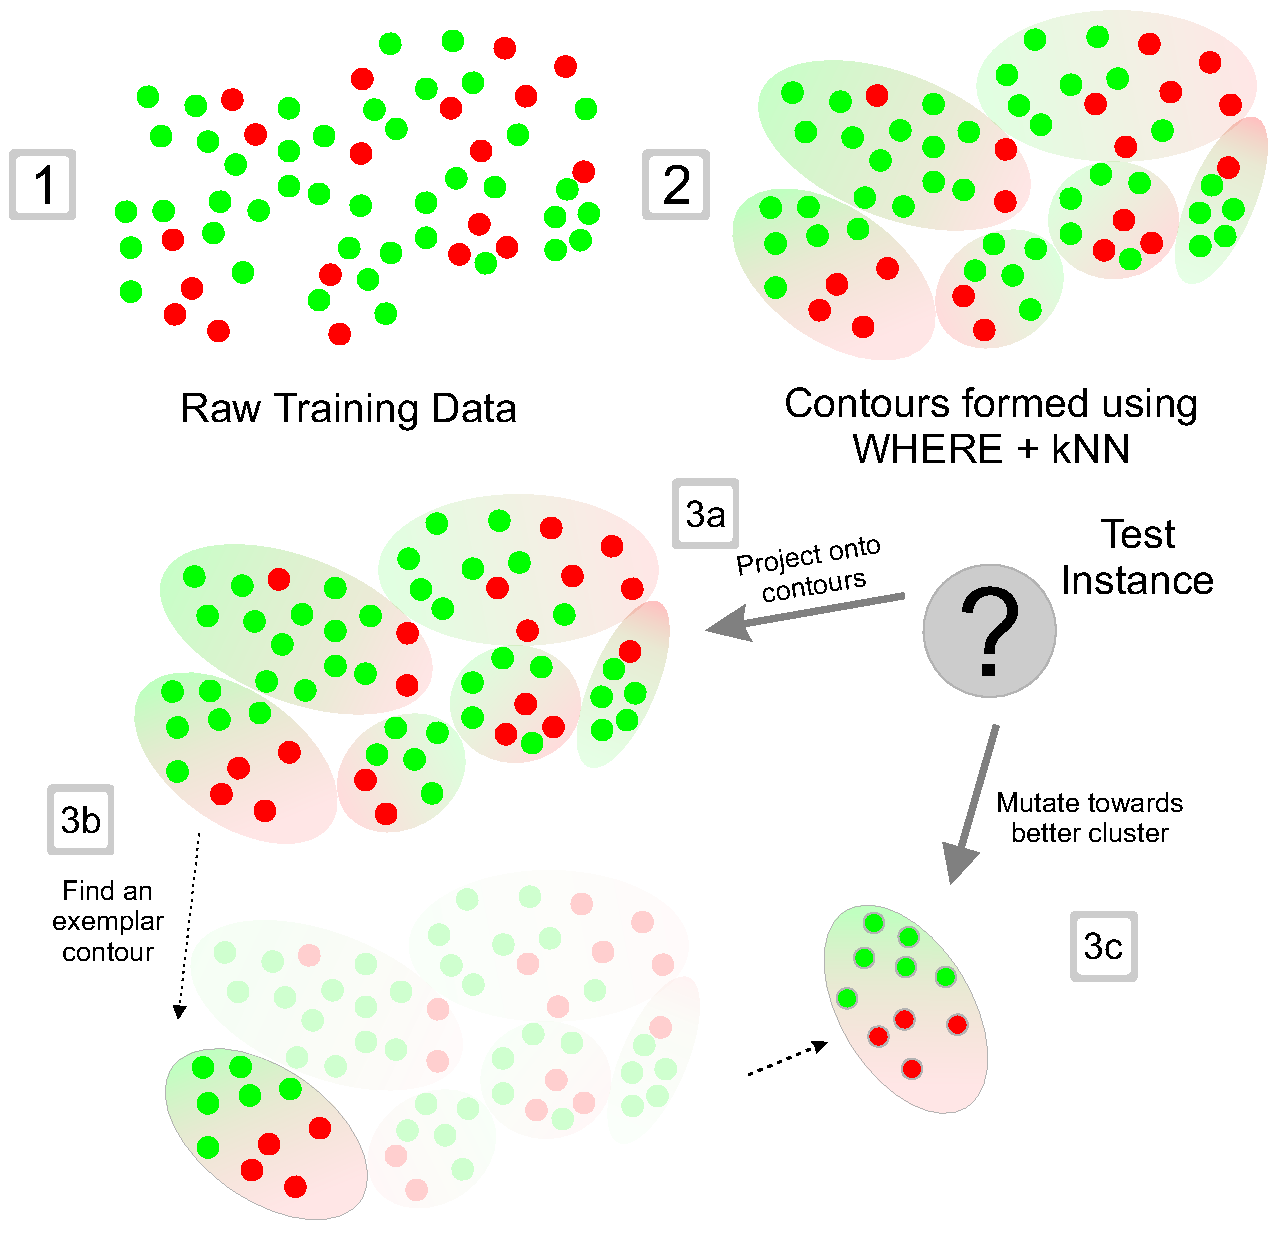
\includegraphics[width=\linewidth]{_figs/WHAT-Clusters2.pdf}
\caption{HERE}
\label{fig:whatflow}
\end{figure}

\begin{figure}[!b]
\begin{python}[left]
def fastmap(data): 
  """Project data on a line 
     between 2 dist points
  """
  z          = random.choose(data)
  east       = furthest(z, data)
  west       = furthest(east, data)
  data.poles = (west,east)
  c          = dist(west,east)     
  for one in data.members: 
    one.pos = project(west,east,c,one)
  data = sorted(data) # sorted by 'pos'
  return split(data)

def project(west, east, AC, x): 
  "Project x onto line east to west"
  AB = dist(x,west)
  BC = dist(x,east)
  #cosine rule
  return (AB$^2$ + AC$^2$ - AB$^2$)/(2*AC) 

def furthest(x,data): 
  # what is furthest from x?
  out, max = x,0
  for y in data:
    d = dist(x,y)
    if d > max: out, max = y, d
  return out

def split(data): # Split at median
   mid = len(data)/2; 
  return data[mid:], data[:mid]

def WHERE(data, scores={}, 
          lvl=10000, prune=True):  
  "Recursively split data."
  if lvl < 1: 
     return data # stop if out of levels
  leafs      = [] # Empty Set
  left,right = fastmap(data)
  west, east = data.poles
  $\omega=\sqrt{\mu}$ # enough data for recursion
  goWest = len(left) > $\omega$  
  goEast = len(right) > $\omega$ 
  if prune: 
    if goEast and better(west,east,scores): 
       goEast = False 
    if goWest and better(east,west,scores): 
       goWest = False 
  if goWest:  
     leafs += where(left,  lvl - 1, prune)  
  if goEast:  
     leafs += where(right, lvl - 1, prune) 
  return leafs

\end{python}
\caption{Clustering with WHERE}
\label{fig:fastmapCode}   
\end{figure}


\begin{figure}[!t]
\begin{python}[right]
def envied(leaves):
  """
  Returns a single exemplary row from 
  a cluster.
  """

def fWeight(train, prune = 0):
  """
  Find the feature weights & prune features
  """

def getContours(train):
  """
  Identify the pairs of clusters
  that can form a contour
  """
  contours = []
  # Clustering with where
  clusters = WHERE(train) 
  near = lambda x: knn(x, clusters)[1]
  for c in clusters:
    one = envied(c)
    two = envied(near(one, clusters))
    contours += [(one, two)]
  return contours

def project(a, b, test):
  if score(a) > score(b):
    good, bad = a,b 
  else:
    good, bad = b,a
  AB = dist(bad,test)
  BC = dist(good,test)
  AC = dist(good,bad)
  # Cosine rule
  x = (AB$^2$ + AC$^2$ - BC$^2$)/(2*AC)
  return $\sqrt{AB^2 - x^2}$

def mutate(me, others, weights = None):
  "Mutate 'me' towards 'others'"
  if weights:
    return [my + ext * f * (good - my) for 
    f, my, good in zip(wights, me, others)]
  else:
    return [my + ext * (good - my) 
    	 for my, good in zip(me, others)]

def nearestContour(contours, instance):
  "Find the nearest contour to an instance"
  return sorted(
        contours,
        key=lambda F: project(
        F[0], F[1], instance), 
        reverse=True)[0]
        
def HERE():
  contours = getContours()
  weights = fWeight(train)
  for rows in defectiveRows:
    vtx = nearestContour(contours, rows)
    [good, bad] = sorted(vtx
            , key=lambda F: score(F))
    new += mutate(rows, good, weights)
  return new
\end{python}
\caption{Instance-based Planning using HERE}
\label{fig:HERE}   
\end{figure}

\subsection{Defect Prediction}

To validate the treatments that have been suggested by our planner, we need to have defect predictors that capable of identifying if a certain module may (or may not) have a defect. A recent IEEE TSE paper by Lessmann et al.~\cite{lessmann} compared 21 different learners for software defect prediction: 
\bi
\item
{\em Statistical classifiers:}
Linear    discrimin analysis,
Quadratic discrimin analysis,
Logistic regression,
Naive Bayes,
Bayesian networks,
Least-angle regression,
Relevance vector machine,

\item
{\em Nearest neighbor methods:}
k-nearest neighbor,
K-Star

\item
{\em Neural networks:}
Multi-Layer Perceptron,
Radial bias functions,

\item
{\em Support vector machine-based classifiers:}
Support vector machine,
Lagrangian SVM
Least squares SVM,
Linear programming,
Voted perceptron,

\item
{\em Decision-tree approaches:}
C4.5,
CART,
Alternating DTs
\item
{\em Ensemble methods:}
\textbf{Random Forest},
Logistic Model Tree.
\ei

They concluded that Random Forrest was the best method, CART being the worst.

Random Forest is an ensemble learning scheme that constructs a number of decision trees at the training time, for a test instance it outputs the mode of the classes of individual tree. It's patent from how random forest operates that the prediction will suffer if there is an imbalance in classes during the training. Unfortunately, the data sets explored here do suffer from severe skewness, as highlighted in~\ref{fig:classimb}. A study conducted by Pelayo and Dick~\cite{smote2} inspected this issue. They showed that the SMOTE technique~\cite{smote} can be used to improve recognition of defect-prone modules. 

In short, SMOTE works by under-sampling the majority class and oversampling all the minority classes in the training data. We use a similar approach with one minor addition to the original algorithm. In our implementation of SMOTE we have introduced an additional step called \textit{resampling}, wherein we ensure that after we do the over/under sampling, the new training data does not have any of the original rows. The new training data merely resembles the original data. This is done as a precautionary measure, so as not to have HERE and Random Forest train on the same training data. 
%Its worth noting that both HERE and Random Forest require some data to train. In order to prevent the two from using the same data to train, we run SMOTE by  \textit{resampling} the classes. Re-sampling 

\begin{figure*}[htbp!]
  \renewcommand{\baselinestretch}{0.8}\begin{center}
    {\scriptsize
      \begin{tabular}{c|l|p{4.7in}}
        amc & average method complexity & e.g. number of JAVA byte codes\\\hline
        avg\, cc & average McCabe & average McCabe's cyclomatic complexity seen
        in class\\\hline
        ca & afferent couplings & how many other classes use the specific
        class. \\\hline
class. \\\hline
        cam & cohesion amongst classes & summation of number of different
        types of method parameters in every method divided by a multiplication
        of number of different method parameter types in whole class and
        number of methods. \\\hline
        cbm &coupling between methods &  total number of new/redefined methods
        to which all the inherited methods are coupled\\\hline
        cbo & coupling between objects & increased when the methods of one
        class access services of another.\\\hline
        ce & efferent couplings & how many other classes is used by the
        specific class. \\\hline
        dam & data access & ratio of the number of private (protected)
        attributes to the total number of attributes\\\hline
        dit & depth of inheritance tree &\\\hline
        ic & inheritance coupling &  number of parent classes to which a given
        class is coupled (includes counts of methods and variables inherited)
        \\\hline
        lcom & lack of cohesion in methods &number of pairs of methods that do
        not share a reference to an instance variable.\\\hline
        locm3 & another lack of cohesion measure & if $m,a$ are  the number of
        $methods,attributes$
        in a class number and $\mu(a)$  is the number of methods accessing an
        attribute, 
        then
        $lcom3=((\frac{1}{a} \sum, j^a \mu(a, j)) - m)/ (1-m)$.
        \\\hline
        loc & lines of code &\\\hline
        max\, cc & maximum McCabe & maximum McCabe's cyclomatic complexity seen
        in class\\\hline
        mfa & functional abstraction & number of methods inherited by a class
        plus number of methods accessible by member methods of the
        class\\\hline
        moa &  aggregation &  count of the number of data declarations (class
        fields) whose types are user defined classes\\\hline
        noc &  number of children &\\\hline
        npm & number of public methods & \\\hline
        rfc & response for a class &number of  methods invoked in response to
        a message to the object.\\\hline
        wmc & weighted methods per class &\\\hline
        \rowcolor{lightgray}
        defect & defect & Boolean: where defects found in post-release bug-tracking systems.
      \end{tabular}
    }
  \end{center}
  \caption{OO measures used in our defect data sets.  Last line is
    the dependent attribute (whether a defect is reported to  a
    post-release bug-tracking system).}\label{fig:ck}
\end{figure*}

\begin{figure}[!tb]
  \renewcommand{\baselinestretch}{0.8}\begin{center}
{\scriptsize
\begin{tabular}{l@{~~~}l@{~~~}l@{~~~}l@{~~~}l@{~~~}l@{~~~}l@{~~}}
  \hline
  \rowcolor{lightgray}
  Data & Symbol & Training & Testing & Training Samples& Defective &\% Defective \\\hline

Ant & ant & 1.5, 1.6  &1.7 & 644&124&19.25\\

Camel & cam & 1.2, 1.4 & 1.6 & 1480&361 & 24.39\\

Ivy & ivy & 1.1, 1.4 & 2.0  & 352 & 79 & 22.44\\

Jedit & jed & 4.1, 4.2 & 4.3 & 679 & 127 & 18.70\\

Log4j & log & 1.0, 1.1 & 1.2 & 244 & 71 & 29.09\\

Lucene & luc & 2.0, 2.2 & 2.4 & 442 & 235 & 53.16\\

Poi & poi & 2.0, 2.5 & 3.0 & 699 & 285 & 40.77\\

Synapse & syn & 1.0, 1.1 & 1.2 & 379 & 76 & 20.05\\

Velocity & vel & 1.4, 1.5 & 1.6 & 410& 289 & 70.48\\

Xalan & xal &2.5, 2.6 &2.7 & 1688 & 798 & 47.27\\\hline
\end{tabular}}
\end{center}
\caption{Attributes of the defect datasets}\label{fig:ck}
\end{figure}

\begin{figure}[!hbp]
  \renewcommand{\baselinestretch}{1}\begin{center}
{\scriptsize
\begin{tabular}{llllll}
  \hline
  \rowcolor{lightgray}
Project & Domain & Lang. & LOC & Features & Config\\\hline

Berkeley DB CE & Database & C & 219,811 & 18 & 2560\\

Berkeley DB JE & Database & Java & 42,596 & 32  & 400\\

Apache & Web Server & C & 230,277 & 9 & 192\\

SQLite & Database & C & 312,625 & 39 & 3,932,160\textsuperscript{*}\\

LLVM & Compiler & C++ & 47,549 & 11 & 1024\\

x264 & Video Enc. & C& 45,743 & 16 & 1152\\\hline
\end{tabular}}\par\medskip

{ \footnotesize $^*$ Dataset contains 4, 553 configurations for prediction modeling and 100 additional random configurations for prediction evaluation, see \cite{vapp}.}
\end{center}

\caption{Attributes of the Performance Prediction data sets}\label{fig:cpm}
\end{figure}



\begin{figure}[tbp!]
% \subfloat[\label{oracle}]{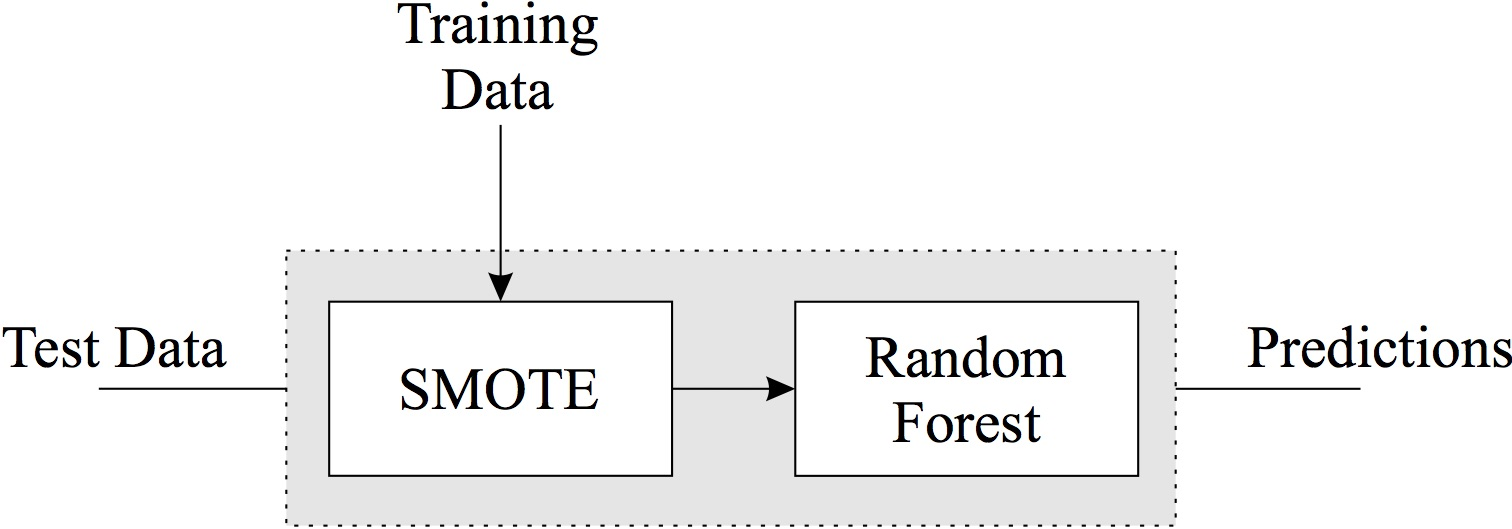
\includegraphics[width=\linewidth]{{_figs//Oracle}}\\
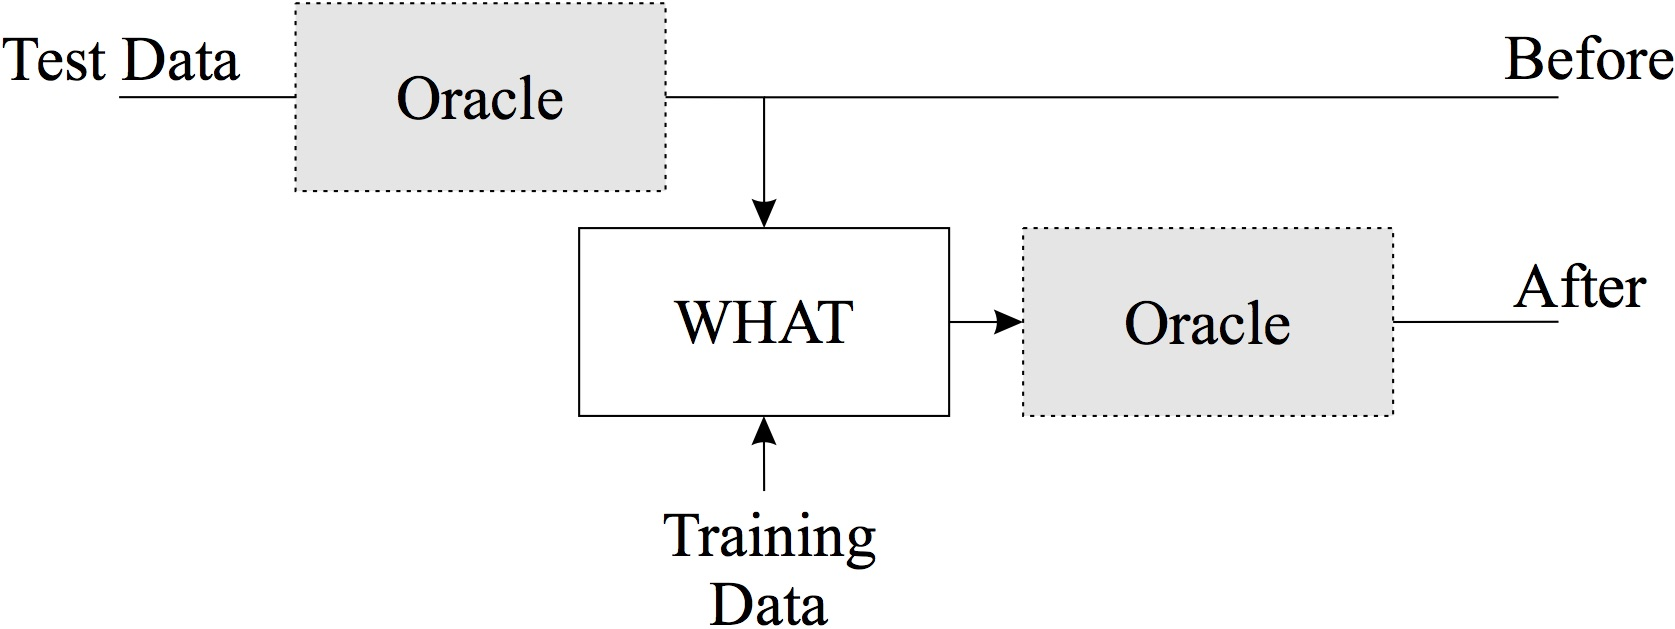
\includegraphics[width=\linewidth]{_figs/WHAT}
\caption{Experimental Rig}
\label{fig:rig}
  
  
%   \subfloat[Experimental Rig for Defect Prediction]{  \includegraphics[width=\linewidth]{_figs/HERE}
%   \label{fig:rig2}}

\end{figure}

%involves two key components. Firstly, there is the oracle (Random Forest with SMOTE) which is used to make predictions. Then we have the 
\section{Data sets}

The following section describes the experimental rig and the experiments used to measure the performance of HERE on 10 defect data sets and 6 performance prediction data sets.

\subsection{Defect Data Set}
The data was obtained from the PROMISE repository\footnote{Promise Repository: \url{openscience.us/repo}}. For the defect data we investigated 32 releases from 11 open source Java projects defined by the metrics highlighted in figure ~\ref{fig:ck}: \kw{Apache Ant} (1.5 -- 1.7), \kw{Apache Camel} (1.2 -- 1.6), \kw{Apache Ivy} (1.1 -- 2.0), \kw{JEdit} (4.1 -- 4.3), \kw{Apache Log4j} (1.0 -- 1.2), \kw{Apache Lucene} (2.0 -- 2.2), \kw{PBeans} (1.0 and 2.0), \kw{Apache POI} (2.0 -- 3.0), \kw{Apache Synapse} (1.0 -- 1.2), \kw{Apache Velocity} (1.4 -- 1.6), and \kw{Apache Xalan-Java} (2.5 -- 2.7). 

Given the empirical nature of the data, it is import to design an experiment such that the planning phase uses only the \kw{past} data to learn trends which can then be applied to the \kw{future} data. Thus for our experiment we use data sets that have at least two consecutive releases. 
\begin{itemize}
\item To generate recommendations for a release $i$, the planner uses releases releases $(i-1)$ and $(i-2)$.
\item The predictor also uses releases $(i-1)$ and $(i-2)$. However, we use SMOTE with re-sampling in order to handle the class imbalance in the data and to prevent the predictor from using the same training data as the planner.
\end{itemize}

\subsection{Performance Prediction Data Set}

{\bfseries RQ3} asks if the aforementioned method can be expanded to other kinds of data. To answer this, we have used the performance prediction data set collected by Siegmund et al. for their ICSE '12 paper~\cite{sven12}. The data sets have been deployed as a part of the \textsc{SPLConqueror} tool\footnote{\url{fosd.de/SPLConqueror}}. This data set contains six examples of real world configurable systems that cover a broad spectrum of scenarios, see figure \ref{fig:cpm} for a summary. The systems have different characteristics (lines of code: 40 thousand to 300 thousand; Valid configurations: 192 to about 3.9 million), different implementation languages (C, C++, and Java), different mechanism (conditional compilation, configuration files, and command-line options), and different domains (Web servers, compilers, encoders, and databases). The data contains a measurement of all the configurations that are invoked by the benchmarking tool. The measurements were conducted 5 to 20 times and the mean of all measurements for each configuration was recoded.

For our experiments, we randomly split the data sets into two equal halves, one for training and the other for testing. The planning phase learns configuration settings from the training half and plans for changes in the test half aiming to optimize the performance of the test instances. We repeat our measurements 20 to 25 times to overcome measurement bias.
\section{Experimental Design}

\subsection{The Rig}

The experimental rig for defect prediction is shown in Figure \ref{fig:rig}. It works as follows: 
\bi
\item We use an {oracle} (Random Forest + SMOTE) to determine whether a certain test case is defective or not. 
\item If the oracle suggests that an instance is defective, then we use HERE to apply the recommendations to that test instance. 
\item The oracle is then used to predict the attributes in the modified instance.
\item The statistical significance of the changes are verified using the cliffs delta measure described below.
\ei

For run time optimization, we use a similar rig. The oracle is Random Forest, and it predicts for run times of specific configuration. HERE is used to generate a recommended configuration to reduce the run times. The run time is measured by the oracle. The reduction of run times are expressed as fractions of the original (also referred to as baseline) run time.

Note that we report the performance scores as a comparison between the oracle's prediction \textit{before} and that \textit{after}. We refrain from using the \textit{actual} defects in the data sets to perform the same comparison. This is because the oracle is limited in its ability to predict defects, there are instances that are inherently misclassified. These misclassifications however are not affected by the planner. Therefore, by comparing the defect counts before and after applying the planner and doing so with a the same oracle would give us an accurate albeit relativistic measure of performance.


\subsection{Performance Assessment}

In order to assess the performance of the planner for the defect data set, we use the Cliffs Delta score to measure the probability that the number of bugs in test data before applying the planner is larger than after doing so. In other words, we use the delta score to measure the ability of the planner to effective reduce the number of defects. Given the untreated test instance labeled \textit{Before} of length \textit{M} and the treated instances labeled \textit{After}, the delta score is obtained as follows:
\begin{equation}
\delta = \frac{\#(Before<After) - \#(Before>After)}{M^2}
\label{eq:cliffs}
\end{equation}

In the context of our application, the $\delta$ attains a value of -1 if the number of defects after applying the treatments has reduced to zero. On the other hand $\delta$ will be 0 if there is no change at all. Thus, most of the values reported will lie between 0 and -1. It needs to be highlighted that although $\delta$ can lie between -1 and +1, the in our application the range is limited to -1 and 0. And this is because we only apply the treatments to defective cases. 

For the performance prediction data set on the other hand, Cliff's delta measure is not directly applicable. We therefore assess the performance by measuring the gain, given by $\frac{Before}{After}$. The gain takes a value larger than 1 if the run times have been reduced, a value of 1 if there is no change, and a value less than 1 if run times have increased after applying the recommended changes. 

In addition to the above, we rank the different various of the planning scheme to identify the best approach. We make use of the Scott-Knott procedure, recommended by Mittas \& Angelis in their 2013 IEEE TSE paper~\cite{sk}, to compute the ranks. It works as follows: A list of treatments \textit{l} is sorted by the Median score. The list \textit{l} is then split into sub-lists m, n in order to maximize the expected value of the differences in the observed performance before and after division. A statistical hypothesis test \textit{H} is applied on the splits \textit{m, n} to check if they are statistically different. If so, Skott-Knott then recurses on each division. 

The research conducted by Shepperd and MacDonell~\cite{shepperd12a}, Kampenes~\cite{kampenes07} and Kocaguenli et al.~\cite{}, highlighted that an ``effect size'' in lieu of a mere hypothesis test is required in order to verfiy if two populations are ``significly'' different. An ICSE'11 paper by Arcuri~\cite{} endorsed the use of Vargha and Delaney's A12 effect size for reporting results in software engineering. Thus, for hypothesis testing H in Skott-Knott, we use the A12 test and a non-parametric bootstrap sampling~\cite{}.

\section{Experimental Results}

\subsection{Defect Data Set}
This sections explores \textbf{RQ2: Can lessons learnt from local policy generators be useful for generating solutions that can be used to mitigate defects in software systems?}

Figure \ref{fig:bugs} compares the number of defects before and after applying "HERE". The graphs represent the median scores, with the inter-quartile ranges represented by the error bars. The results seem to show that in all data sets under consideration, the number of defects have reduced, some more so than others. Large differences were notice in certain data sets namely, \textit{ant}, \textit{camel}, \textit{jedit}, \textit{poi,} and \textit{xalan}, on close examination it was noticed that these data sets had comparatively large training data, which translates to more samples for the planner to learn from.

In addition to this, to study the statistical significance of the changes, the results were statistically verified using the Skott-Knott procedure. In order to do this we computed the Cliff's Delta score. As highlighted previously, HERE is applied only for test instances that are considered defective by the oracle. Using \eq{cliffs} we can expect to see the following results:

\bi
\item $\lt$ 0 if defects have been suppressed.
\item = 0 if no change has been made.
\item $\gt$ 0 if new defects have been introduced. This is not applicable to our case because we only apply HERE to defective cases; either the defects are suppressed or they remain unaltered, introduction of new defects is not possible.
\ei


\begin{figure}[tbp]
\centering
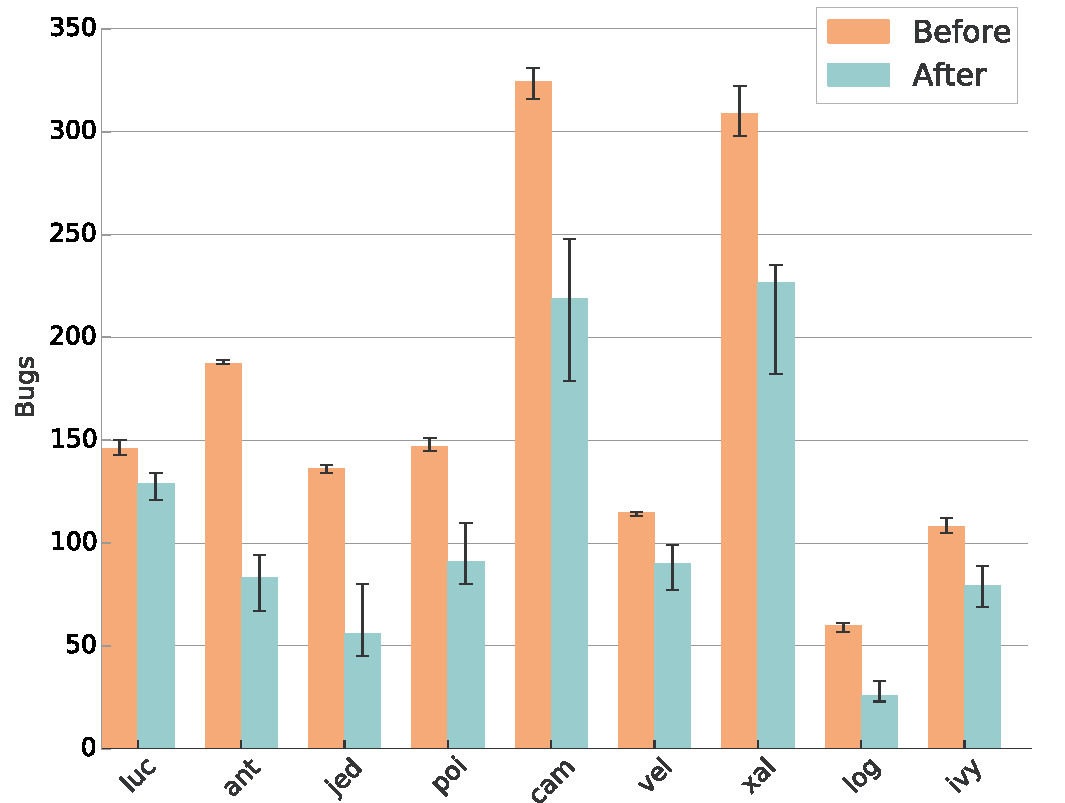
\includegraphics[width=\linewidth]{_figs/histograms.pdf}
\caption{Comparison of defects before and after planning.}
\label{fig:bugs}
\end{figure}
With this in mind, it is easy to note that lower cliffs delta score translates to better the performance. 

 
The results are tabulated in figure \ref{tab:ant}. For the sake of completeness, we have introduced three basic configurations in HERE: 
\bi
\item \textit{Extent of Mutation:} Denotes the extent by which a test instant is \textit{mutated} towards the best cluster in the contour. It is a fraction that lies between 0 and 1. The baseline study requires no change be made, and thus extent of mutation is set to zero.
\item \textit{Feature Weighting:} The importance of feature weighting has already been discussed in section \ref{fwt}. It is a fraction that lies between 0 and 1, with 0 being the least important and 1 the most important feature. The extent of mutation is multiplied by this fraction to determine how much a specific feature changes by. Generally, we would like to make the largest change to the most crucial feature.
\item \textit{Information Pruning:} In addition to the weighting the features, we explored the possibility of mutating only the most important features. The feature weights are already known to us, we sort the features in descending order of their weights and mutate only the first X\%.
\ei
It is to be noted however that 


\begin{figure*}[htbp!]

\noindent\begin{minipage}{0.5\textwidth}
  {\scriptsize \textbf{Ant}\\}
  {\scriptsize  \begin{tabular}{{l@{~~~~}l@{}r@{~~~~}r@{~~~~}c}}
      \arrayrulecolor{darkgray}
      \rowcolor[gray]{.9} \textbf{Rank} & \textbf{Treatment} & \textbf{Median} & \textbf{IQR} & \\
  1 & 0.75 &    -0.63  &  0.08 & \quart{2}{7}{5}{144} \\
  1 & 0.75, weighting &    -0.6  &  0.2 & \quart{0}{16}{8}{144} \\
\hline  2 & 0.5, weighting &    -0.42  &  0.11 & \quart{17}{10}{23}{144} \\
  2 & 0.5 &    -0.42  &  0.11 & \quart{19}{9}{23}{144} \\
  2 & 0.75, weighting, Prune=50\% &    -0.4  &  0.11 & \quart{20}{9}{25}{144} \\
\hline  3 & 0.25 &    -0.28  &  0.09 & \quart{31}{7}{35}{144} \\
  3 & 0.25, weighting &    -0.28  &  0.08 & \quart{31}{7}{35}{144} \\
\hline  4 & 0.5, weighting, Prune=50\% &    -0.25  &  0.06 & \quart{35}{5}{38}{144} \\
\hline  5 & 0.25, weighting, Prune=50\% &    -0.19  &  0.05 & \quart{41}{4}{43}{144} \\
\hline  6 & Baseline &    -0.11  &  0.03 & \quart{47}{2}{49}{144} \\
\hline \end{tabular}}
\end{minipage}
\noindent\begin{minipage}{0.5\textwidth}
  \flushleft
  {\scriptsize \textbf{Camel}\\}
{\scriptsize  \begin{tabular}{{l@{~~~~}l@{}r@{~~~~}r@{~~~~}c}}
\arrayrulecolor{darkgray}
\rowcolor[gray]{.9} \textbf{Rank} & \textbf{Treatment} & \textbf{Median} & \textbf{IQR} & \\
  1 &  0.75, weighting, Prune=50\% &    -0.41  &  0.1 & \quart{2}{14}{9}{205} \\
  1 &  0.75 &    -0.41  &  0.23 & \quart{1}{32}{9}{205} \\
  1 &  0.75, weighting &    -0.39  &  0.16 & \quart{0}{22}{12}{205} \\
\hline  2 &  0.5, weighting, Prune=50\% &    -0.27  &  0.09 & \quart{19}{12}{29}{205} \\
  2 &  0.5 &    -0.26  &  0.12 & \quart{20}{17}{30}{205} \\
  2 &  0.5, weighting &    -0.24  &  0.09 & \quart{24}{13}{33}{205} \\
\hline  3 &  0.25, weighting, Prune=50\% &    -0.2  &  0.05 & \quart{36}{7}{38}{205} \\
  3 &  0.25, weighting &    -0.19  &  0.07 & \quart{36}{9}{40}{205} \\
  3 &  0.25 &    -0.17  &  0.06 & \quart{37}{8}{43}{205} \\
\hline  4 &  Baseline &    -0.15  &  0.06 & \quart{41}{8}{45}{205} \\
\hline \end{tabular}}
\end{minipage}

\noindent\begin{minipage}{0.5\textwidth}
  \flushleft
  {\scriptsize \textbf{Ivy}\\[-0.05cm]}
{\scriptsize  \begin{tabular}{{l@{~~~~}l@{}r@{~~~~}r@{~~~~}c}}
\arrayrulecolor{darkgray}
\rowcolor[gray]{.9} \textbf{Rank} & \textbf{Treatment} & \textbf{Median} & \textbf{IQR} & \\
  1 &     0.75 &    -0.57  &  0.17 & \quart{0}{16}{6}{163} \\
  1 &   0.75, weighting &    -0.55  &  0.11 & \quart{3}{11}{8}{163} \\
\hline  2 &   0.75, weighting, Prune=50\% &    -0.38  &  0.11 & \quart{19}{11}{25}{163} \\
  2 &    0.5, weighting &    -0.36  &  0.12 & \quart{23}{12}{27}{163} \\
  2 &   0.5 &    -0.33  &  0.11 & \quart{25}{11}{30}{163} \\
\hline  3 &   0.5, weighting, Prune=50\% &    -0.27  &  0.08 & \quart{30}{8}{36}{163} \\
\hline  4 &   0.25, weighting &    -0.2  &  0.07 & \quart{41}{7}{43}{163} \\
  4 &     0.25 &    -0.16  &  0.04 & \quart{43}{4}{47}{163} \\
  4 &     Baseline &    -0.16  &  0.0 & \quart{47}{0}{47}{163} \\
\hline  5 &   0.25, weighting, Prune=50\% &    -0.15  &  0.04 & \quart{45}{4}{48}{163} \\
\hline \end{tabular}}
\end{minipage}
\noindent\begin{minipage}{0.5\textwidth}
  \flushleft
  {\scriptsize \textbf{Jedit}\\}
  {\scriptsize  \begin{tabular}{{l@{~~~~}l@{}r@{~~~~}r@{~~~~}c}}
\arrayrulecolor{darkgray}
\rowcolor[gray]{.9} \textbf{Rank} & \textbf{Treatment} & \textbf{Median} & \textbf{IQR} & \\
  1 &  0.75, weighting, Prune=50\% &    -0.41  &  0.18 & \quart{0}{20}{8}{172} \\
  1 &  0.75 &    -0.35  &  0.26 & \quart{0}{30}{15}{172} \\
\hline  2 &  0.75, weighting &    -0.25  &  0.17 & \quart{16}{20}{26}{172} \\
  2 &  0.5, weighting, Prune=50\% &    -0.21  &  0.1 & \quart{23}{11}{31}{172} \\
\hline  3 &   0.5 &    -0.17  &  0.08 & \quart{32}{9}{36}{172} \\
  3 &  0.5, weighting &    -0.14  &  0.09 & \quart{31}{10}{39}{172} \\
\hline  4 &  0.25, weighting, Prune=50\% &    -0.12  &  0.06 & \quart{39}{7}{41}{172} \\
\hline  5 &  0.25 &    -0.08  &  0.05 & \quart{43}{5}{46}{172} \\
  5 &  0.25, weighting &    -0.08  &  0.06 & \quart{43}{6}{46}{172} \\
\hline  6 &  Baseline &    -0.06  &  0.01 & \quart{47}{1}{48}{172} \\
\hline \end{tabular}}
\end{minipage}


\noindent\begin{minipage}{0.5\textwidth}
  \flushleft
  {\scriptsize \textbf{Log4j}\\}
  {\scriptsize  \begin{tabular}{{l@{~~~~}l@{}r@{~~~~}r@{~~~~}c}}
\arrayrulecolor{darkgray}
\rowcolor[gray]{.9} \textbf{Rank} & \textbf{Treatment} & \textbf{Median} & \textbf{IQR} & \\
  1 &  0.75, weighting, Prune=50\% &    -0.19  &  0.13 & \quart{0}{28}{15}{273} \\
\hline  2 &  0.75 &    -0.13  &  0.06 & \quart{23}{13}{28}{273} \\
  2 &  0.5, weighting, Prune=50\% &    -0.13  &  0.05 & \quart{23}{11}{28}{273} \\
  2 &  0.75, weighting &    -0.12  &  0.1 & \quart{15}{21}{30}{273} \\
\hline  3 &  0.5, weighting &    -0.1  &  0.03 & \quart{28}{6}{34}{273} \\
\hline  4 &   0.5 &    -0.1  &  0.07 & \quart{28}{15}{34}{273} \\
  4 &  0.25 &    -0.09  &  0.04 & \quart{34}{9}{36}{273} \\
  4 &  0.25, weighting, Prune=50\% &    -0.09  &  0.04 & \quart{34}{9}{36}{273} \\
  4 &  0.25, weighting &    -0.06  &  0.04 & \quart{34}{9}{43}{273} \\
\hline  5 &  Baseline &    -0.06  &  0.03 & \quart{43}{6}{43}{273} \\
\hline \end{tabular}}
\end{minipage}
\noindent\begin{minipage}{0.5\textwidth}
  \flushleft
  {\scriptsize \textbf{Lucene}\\}
  {\scriptsize  \begin{tabular}{{l@{~~~~}l@{}r@{~~~~}r@{~~~~}c}}
\arrayrulecolor{darkgray}
\rowcolor[gray]{.9} \textbf{Rank} & \textbf{Treatment} & \textbf{Median} & \textbf{IQR} & \\
  1 &  0.75, weighting &    -0.15  &  0.09 & \quart{0}{29}{9}{393} \\
  1 &  0.75 &    -0.13  &  0.09 & \quart{0}{29}{16}{393} \\
  1 &  0.75, weighting, Prune=50\% &    -0.12  &  0.08 & \quart{6}{27}{19}{393} \\
\hline  2 &  Baseline &    -0.1  &  0.03 & \quart{26}{10}{26}{393} \\
  2 &  0.5, weighting, Prune=50\% &    -0.1  &  0.03 & \quart{23}{10}{26}{393} \\
\hline  3 &  0.5, weighting &    -0.08  &  0.06 & \quart{23}{20}{33}{393} \\
  3 &  0.25, weighting, Prune=50\% &    -0.07  &  0.03 & \quart{33}{10}{36}{393} \\
  3 &  0.5 &    -0.07  &  0.05 & \quart{29}{17}{36}{393} \\
\hline  4 &  0.25, weighting &    -0.04  &  0.04 & \quart{36}{13}{46}{393} \\
  4 &  0.25 &    -0.04  &  0.02 & \quart{39}{7}{46}{393} \\
\hline \end{tabular}}
\end{minipage}

\noindent\begin{minipage}{0.5\textwidth}
  \flushleft
  {\scriptsize \textbf{Poi}\\}
  {\scriptsize  \begin{tabular}{{l@{~~~~}l@{}r@{~~~~}r@{~~~~}c}}
      \arrayrulecolor{darkgray}
\rowcolor[gray]{.9} \textbf{Rank} & \textbf{Treatment} & \textbf{Median} & \textbf{IQR} & \\
  1 & 0.75, weighting &    -0.45  &  0.1 & \quart{6}{10}{11}{162} \\
  1 &  0.75 &    -0.44  &  0.23 & \quart{0}{23}{12}{162} \\
\hline  2 & 0.5, weighting &    -0.32  &  0.23 & \quart{12}{24}{24}{162} \\
  2 & 0.5 &    -0.26  &  0.23 & \quart{18}{24}{31}{162} \\
  2 & 0.75, weighting, Prune=50\% &    -0.25  &  0.19 & \quart{17}{20}{32}{162} \\
\hline  3 & 0.5, weighting, Prune=50\% &    -0.19  &  0.09 & \quart{34}{9}{38}{162} \\
  3 &  0.25 &    -0.19  &  0.11 & \quart{32}{11}{38}{162} \\
  3 & 0.25, weighting &    -0.17  &  0.14 & \quart{30}{14}{40}{162} \\
\hline  4 & 0.25, weighting, Prune=50\% &    -0.12  &  0.09 & \quart{40}{9}{45}{162} \\
\hline  5 &  Baseline &    -0.09  &  0.03 & \quart{46}{3}{48}{162} \\
\hline \end{tabular}}
\end{minipage}
\noindent\begin{minipage}{0.5\textwidth}
  \flushleft
  {\scriptsize \textbf{Synapse}\\}
  {\scriptsize  \begin{tabular}{{l@{~~~~}l@{}r@{~~~~}r@{~~~~}c}}
\arrayrulecolor{darkgray}
\rowcolor[gray]{.9} \textbf{Rank} & \textbf{Treatment} & \textbf{Median} & \textbf{IQR} & \\
  1 & 0.75, weighting &    -0.56  &  0.2 & \quart{7}{18}{11}{148} \\
  1 & 0.75 &    -0.48  &  0.34 & \quart{0}{29}{18}{148} \\
\hline  2 & 0.5 &    -0.4  &  0.27 & \quart{14}{24}{25}{148} \\
  2 & 0.5, weighting &    -0.37  &  0.17 & \quart{21}{15}{28}{148} \\
\hline  3 & 0.25 &    -0.23  &  0.16 & \quart{31}{14}{40}{148} \\
  3 & 0.25, weighting &    -0.23  &  0.1 & \quart{38}{9}{40}{148} \\
  3 & 0.75, weighting, Prune=50\% &    -0.19  &  0.08 & \quart{40}{7}{43}{148} \\
\hline  4 & 0.25, weighting, Prune=50\% &    -0.17  &  0.08 & \quart{42}{7}{45}{148} \\
  4 & Baseline &    -0.15  &  0.0 & \quart{47}{0}{47}{148} \\
  4 & 0.5, weighting, Prune=50\% &    -0.15  &  0.11 & \quart{40}{9}{47}{148} \\
\hline \end{tabular}}
\end{minipage}

\noindent\begin{minipage}{0.50\textwidth}
  \flushleft
  {\scriptsize \textbf{Velocity}\\}
  {\scriptsize  \begin{tabular}{{l@{~~~~}l@{}r@{~~~~}r@{~~~~}c}}
\arrayrulecolor{darkgray}
\rowcolor[gray]{.9} \textbf{Rank} & \textbf{Treatment} & \textbf{Median} & \textbf{IQR} & \\
  1 & 0.75, weighting &    -0.19  &  0.22 & \quart{1}{34}{21}{207} \\
  1 & 0.75, weighting, Prune=50\% &    -0.15  &  0.13 & \quart{14}{20}{28}{207} \\
  1 & 0.75 &    -0.14  &  0.23 & \quart{0}{35}{29}{207} \\
\hline  2 & 0.5 &    -0.13  &  0.11 & \quart{23}{17}{31}{207} \\
\hline  3 & 0.5, weighting &    -0.1  &  0.08 & \quart{29}{13}{35}{207} \\
  3 & 0.5, weighting, Prune=50\% &    -0.07  &  0.07 & \quart{32}{11}{40}{207} \\
\hline  4 & Baseline &    -0.05  &  0.04 & \quart{43}{6}{43}{207} \\
  4 & 0.25, weighting &    -0.05  &  0.03 & \quart{40}{5}{43}{207} \\
  4 & 0.25 &    -0.04  &  0.02 & \quart{43}{3}{45}{207} \\
  4 & 0.25, weighting, Prune=50\% &    -0.01  &  0.04 & \quart{43}{6}{49}{207} \\
\hline \end{tabular}}
\end{minipage}
\noindent\begin{minipage}{0.50\textwidth}
  \flushleft
  {\scriptsize \textbf{Xalan}\\}
  {\scriptsize  \begin{tabular}{{l@{~~~~}l@{}r@{~~~~}r@{~~~~}c}}
\arrayrulecolor{darkgray}
\rowcolor[gray]{.9} \textbf{Rank} & \textbf{Treatment} & \textbf{Median} & \textbf{IQR} & \\
  1 & 0.75 &    -0.36  &  0.12 & \quart{0}{16}{9}{198} \\
  1 & 0.75, weighting &    -0.3  &  0.17 & \quart{4}{23}{18}{198} \\
  1 &    0.5 &    -0.3  &  0.12 & \quart{9}{17}{18}{198} \\
\hline  2 & 0.5, weighting &    -0.28  &  0.09 & \quart{16}{13}{20}{198} \\
\hline  3 & 0.25, weighting &    -0.23  &  0.1 & \quart{20}{14}{27}{198} \\
  3 & 0.25 &    -0.23  &  0.12 & \quart{20}{17}{27}{198} \\
\hline  4 & 0.25, weighting, Prune=50\% &    -0.14  &  0.07 & \quart{36}{9}{40}{198} \\
  4 & 0.75, weighting, Prune=50\% &    -0.14  &  0.07 & \quart{33}{10}{40}{198} \\
  4 & 0.5, weighting, Prune=50\% &    -0.12  &  0.06 & \quart{37}{8}{43}{198} \\
\hline  5 & Baseline &    -0.08  &  0.02 & \quart{47}{2}{48}{198} \\
\hline \end{tabular}}
\end{minipage}
\caption{Cliffs Delta Scores for the defect data set. The Treatment column, has 3 possible configurations, the first (0.25, 0.50, and 0.75) represents the extent of mutation; weighting represents feature weighting; Prune represents the extent of information pruning.}
\label{tab:ant}
\end{figure*}



\begin{figure*}[htbp!]
\centering
\begin{minipage}{0.30\linewidth}
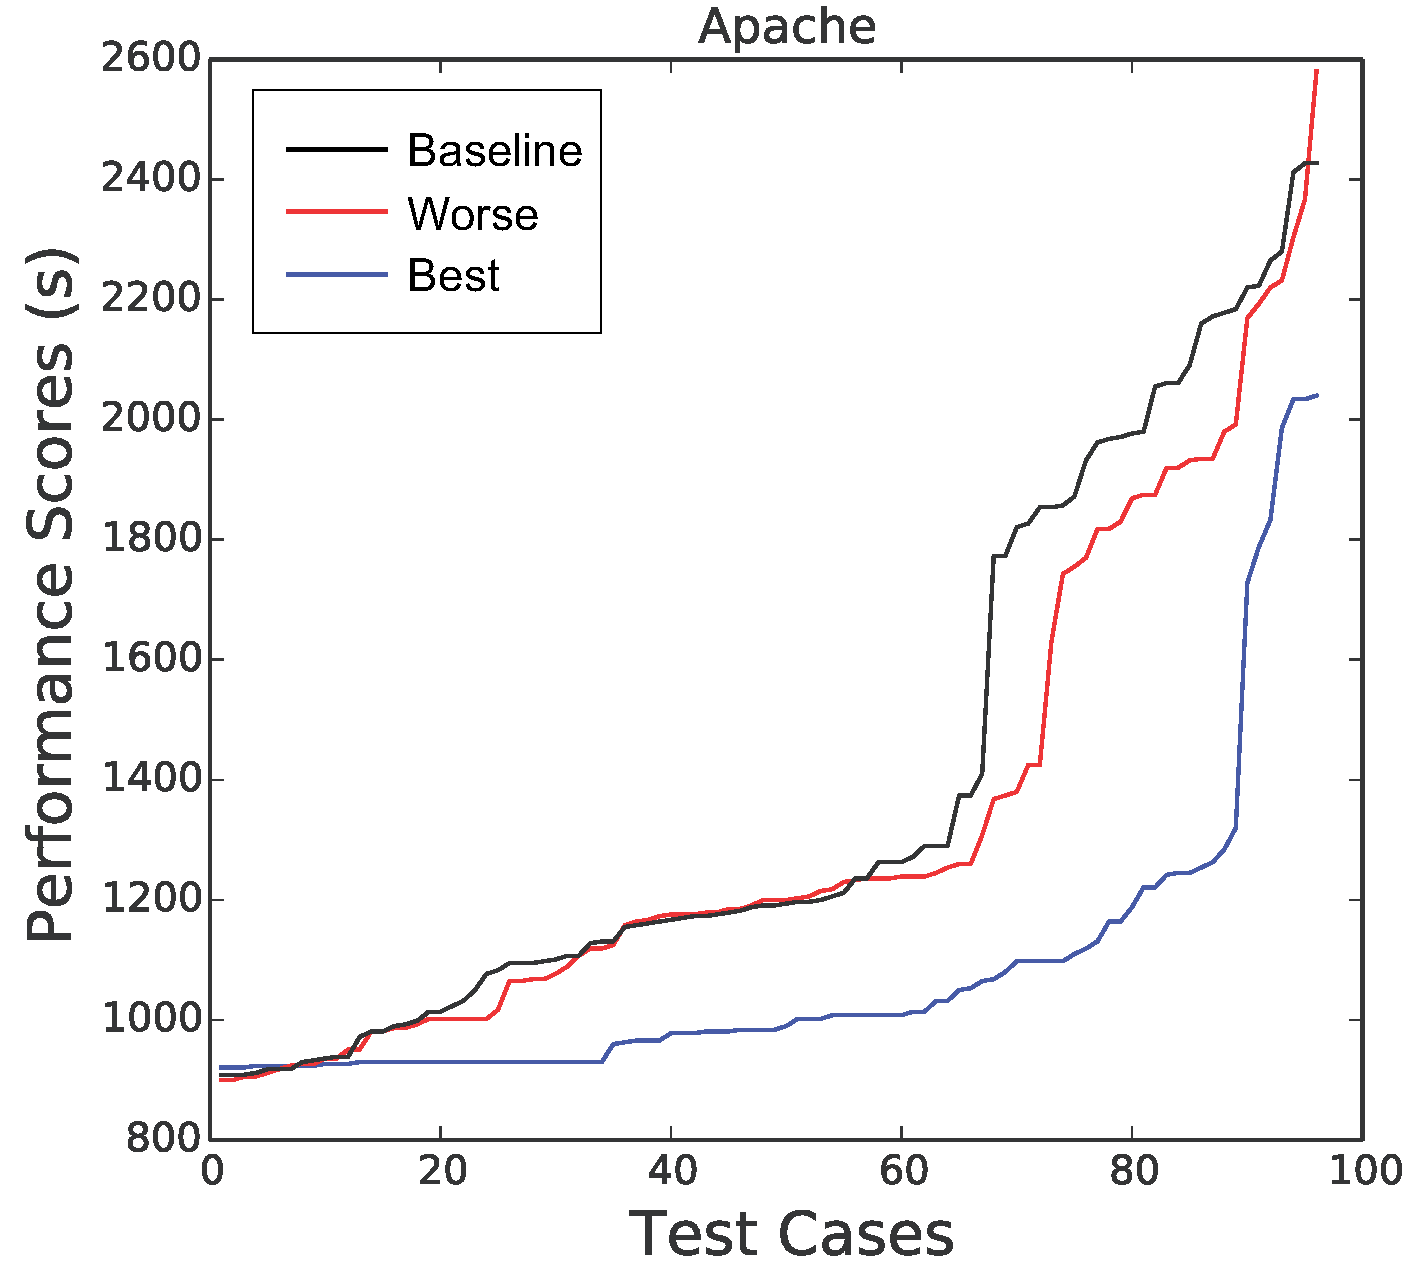
\includegraphics[width=\linewidth]{_figs/Apache.pdf}
\end{minipage}
\begin{minipage}{0.30\linewidth}
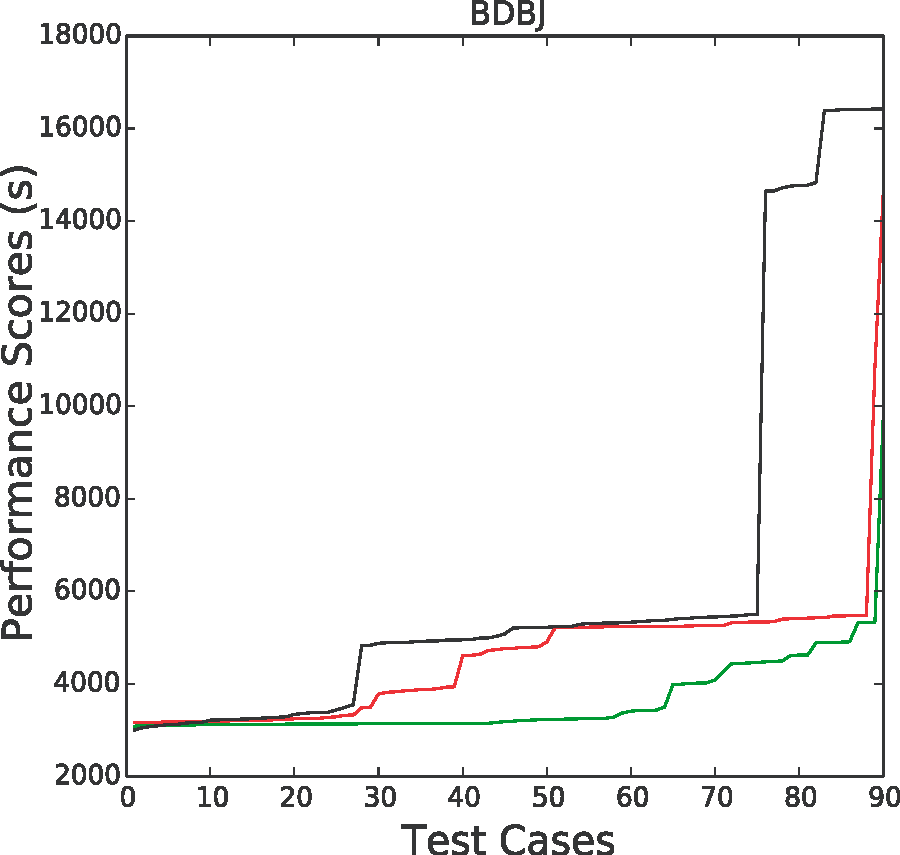
\includegraphics[width=\linewidth]{_figs/BDBJ.pdf}
\end{minipage}
\begin{minipage}{0.30\linewidth}
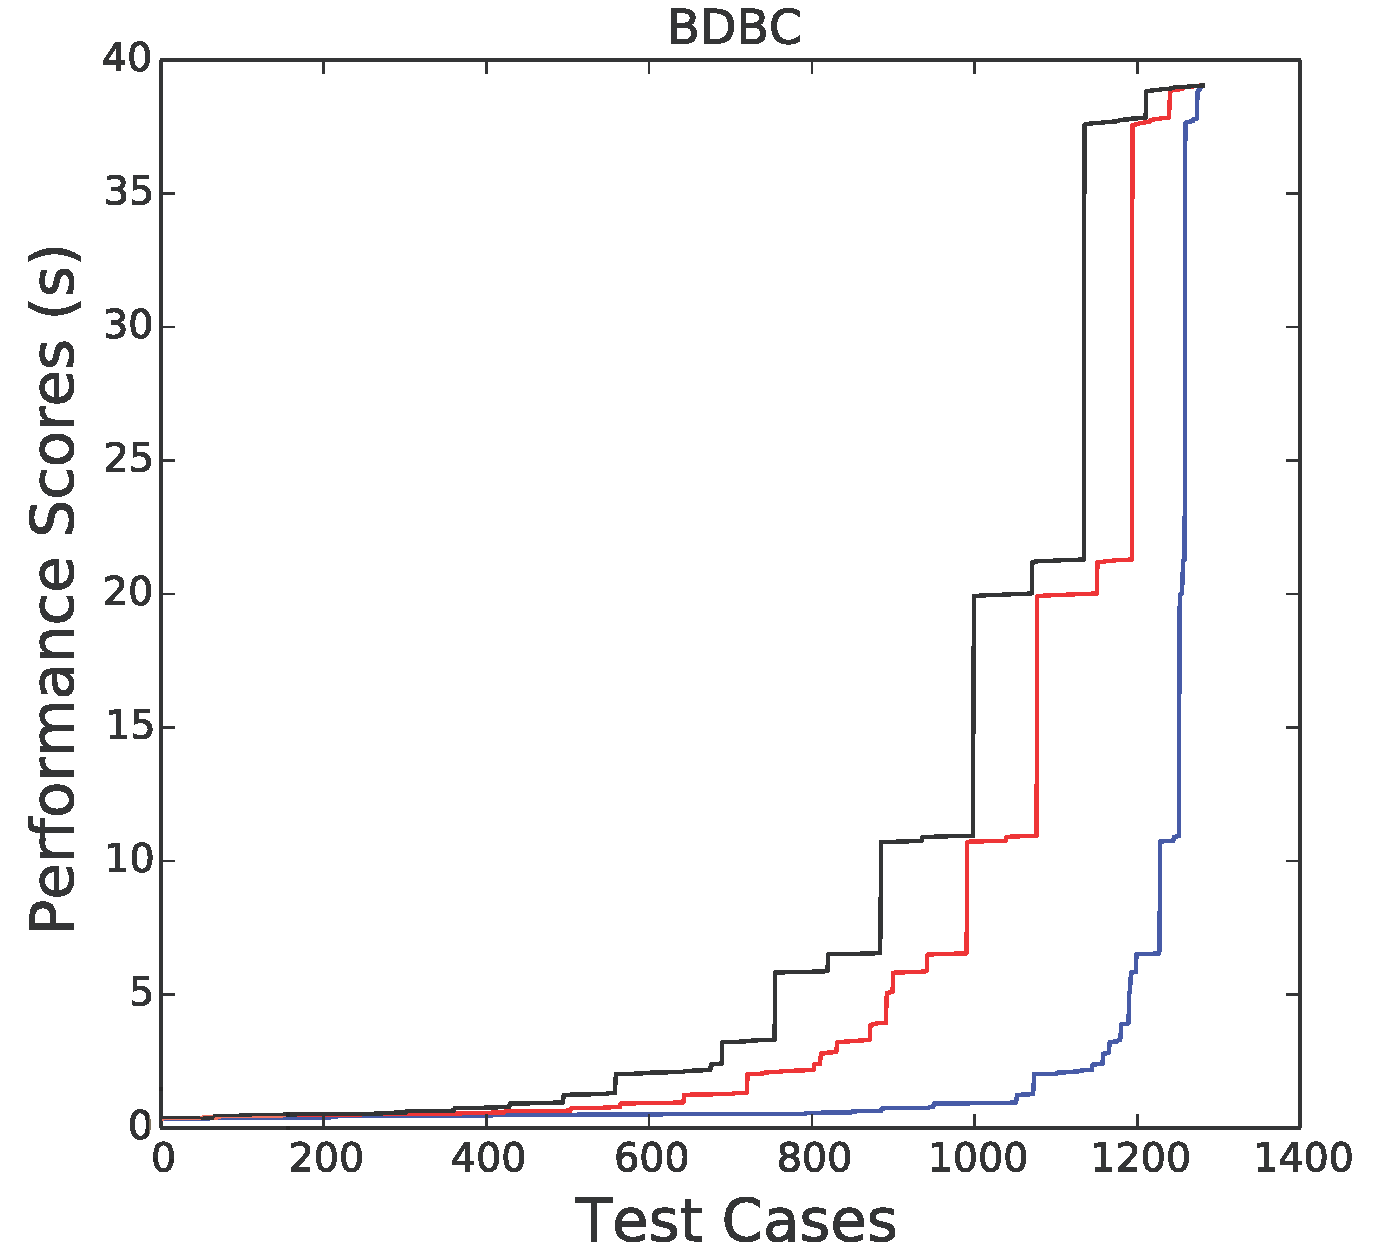
\includegraphics[width=\linewidth]{_figs/BDBC.pdf}
\end{minipage}

\begin{minipage}{0.30\linewidth}
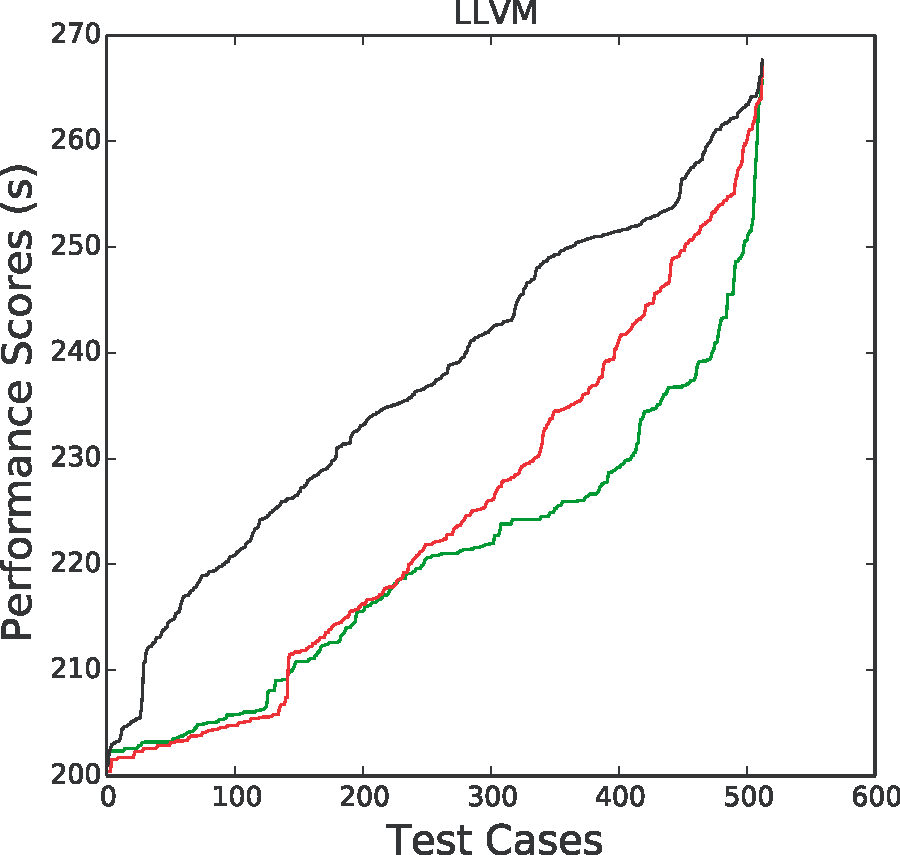
\includegraphics[width=\linewidth]{_figs/LLVM.pdf}
\end{minipage}
\begin{minipage}{0.30\linewidth}
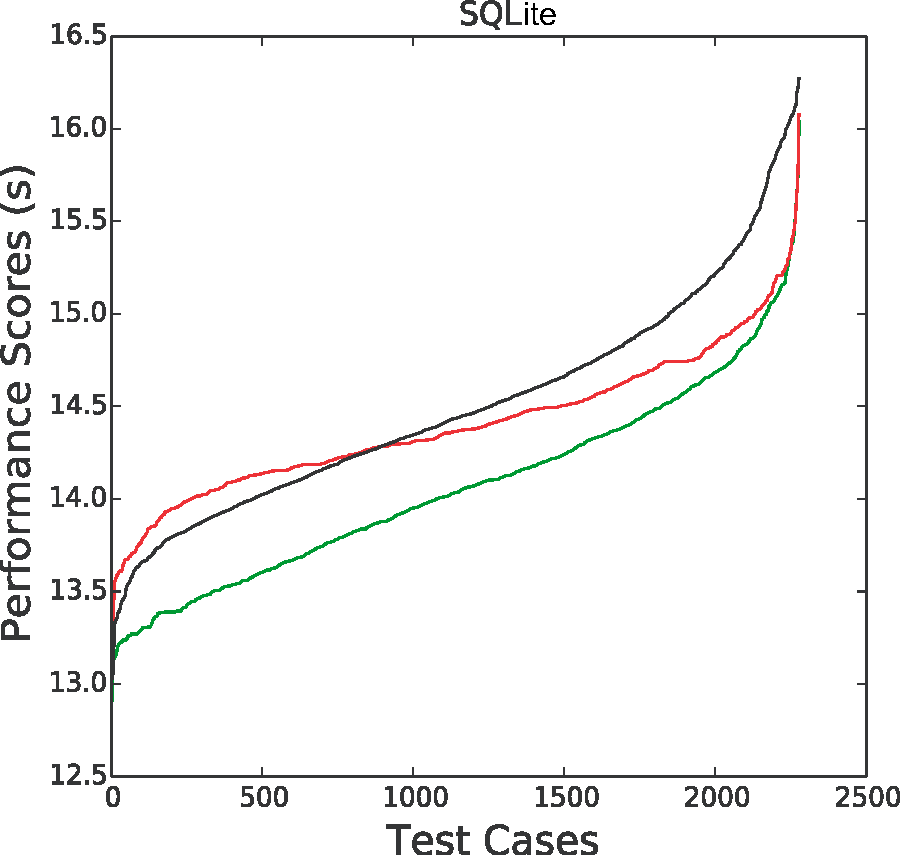
\includegraphics[width=\linewidth]{_figs/SQL.pdf}
\end{minipage}
\begin{minipage}{0.30\linewidth}
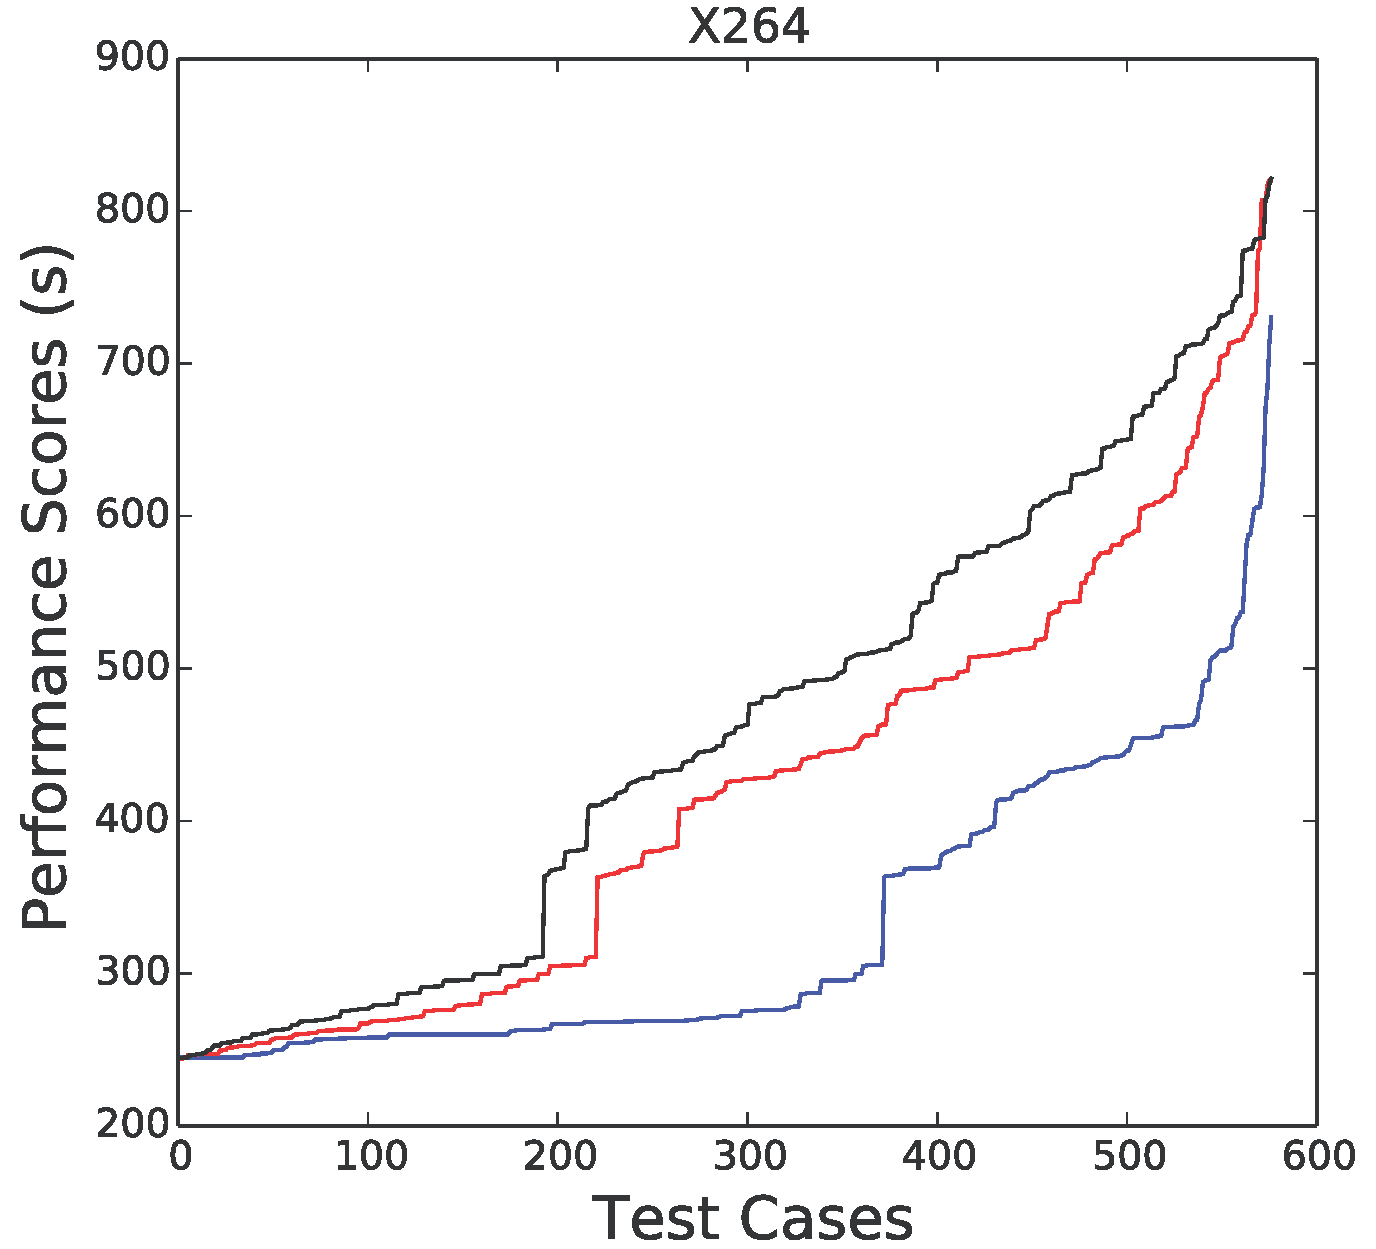
\includegraphics[width=\linewidth]{_figs/X264.pdf}
\end{minipage}
\caption{Run time optimization using HERE. Blue curve represents a mutation probability of 0.75 with feature weighting and information pruning; Red curve represents a mutation probability of 0.25 with feature weighting, but no information pruning; Black curve represents the raw test data used as baseline for the comparison.}
\label{fig:pp}
\end{figure*}


\subsection{Performance Prediction Data set}

In this section, 
\begin{figure*}[htbp!]
\noindent\begin{minipage}{0.5\textwidth}
  {\scriptsize \textbf{Apache}\\}
  {\scriptsize  \begin{tabular}{{l@{~~~~}l@{~~~~}r@{~~~~}r@{~~~~}c}}
      \arrayrulecolor{darkgray}
      \rowcolor[gray]{.9} \textbf{Rank} & \textbf{Treatment} & \textbf{Median} & \textbf{IQR} & \\
  1 & 75, weighting, Prune=25\% &    0.77  &  0.05 & \quart{0}{9}{3}{49} \\
  1 &   75 &    0.79  &  0.08 & \quart{1}{16}{7}{49} \\
\hline  2 & 75, weighting &    0.85  &  0.07 & \quart{9}{14}{19}{49} \\
  2 & 50, weighting, Prune=25\% &    0.85  &  0.04 & \quart{15}{8}{19}{49} \\
  2 &  50 &    0.85  &  0.05 & \quart{17}{10}{19}{49} \\
\hline  3 & 50, weighting &    0.91  &  0.05 & \quart{25}{10}{31}{49} \\
  3 &  25 &    0.92  &  0.04 & \quart{29}{8}{33}{49} \\
  3 & 25, weighting, Prune=25\% &    0.93  &  0.02 & \quart{33}{4}{35}{49} \\
\hline  4 & 25, weighting &    0.96  &  0.03 & \quart{37}{6}{41}{49} \\
\hline  5 & baseline &    1.0  &  0.0 & \quart{49}{0}{49}{49} \\
\hline \end{tabular}}
\end{minipage}
\noindent\begin{minipage}{0.5\textwidth}
  \flushleft
  {\scriptsize \textbf{BDBC}\\}
{\scriptsize  \begin{tabular}{{l@{~~~~}l@{~~~~}r@{~~~~}r@{~~~~}c}}
\arrayrulecolor{darkgray}
\rowcolor[gray]{.9} \textbf{Rank} & \textbf{Treatment} & \textbf{Median} & \textbf{IQR} & \\
  1 &     75 &    0.22  &  0.05 & \quart{0}{3}{1}{49} \\
  1 &  75, weighting, Prune=25\% &    0.21  &  0.04 & \quart{0}{2}{0}{49} \\
\hline  2 &  75, weighting &    0.24  &  0.1 & \quart{0}{6}{2}{49} \\
\hline  3 &     50 &    0.4  &  0.04 & \quart{11}{2}{12}{49} \\
  3 &  50, weighting, Prune=25\% &    0.4  &  0.05 & \quart{10}{3}{12}{49} \\
\hline  4 &  50, weighting &    0.47  &  0.09 & \quart{14}{5}{16}{49} \\
\hline  5 &     25 &    0.66  &  0.03 & \quart{28}{1}{28}{49} \\
  5 &  25, weighting, Prune=25\% &    0.67  &  0.06 & \quart{28}{3}{29}{49} \\
\hline  6 &  25, weighting &    0.69  &  0.06 & \quart{29}{4}{30}{49} \\
\hline  7 &  baseline &    1.0  &  0.0 & \quart{49}{0}{49}{49} \\
\hline \end{tabular}}
\end{minipage}

\noindent\begin{minipage}{0.5\textwidth}
  \flushleft
  {\scriptsize \textbf{BDBJ}\\}
{\scriptsize  \begin{tabular}{{l@{~~~~}l@{~~~~}r@{~~~~}r@{~~~~}c}}
\arrayrulecolor{darkgray}
\rowcolor[gray]{.9} \textbf{Rank} & \textbf{Treatment} & \textbf{Median} & \textbf{IQR} & \\
  1 &     75 &    0.63  &  0.16 & \quart{0}{19}{3}{49} \\
  1 &  75, weighting, Prune=25\% &    0.68  &  0.17 & \quart{1}{21}{9}{49} \\
  1 &  75, weighting &    0.74  &  0.11 & \quart{8}{14}{17}{49} \\
\hline  2 &  50, weighting, Prune=25\% &    0.75  &  0.09 & \quart{14}{12}{18}{49} \\
  2 &     50 &    0.79  &  0.13 & \quart{16}{16}{23}{49} \\
\hline  3 &  50, weighting &    0.82  &  0.09 & \quart{23}{11}{27}{49} \\
\hline  4 &  25, weighting, Prune=25\% &    0.87  &  0.07 & \quart{29}{9}{33}{49} \\
\hline  5 &     25 &    0.88  &  0.06 & \quart{33}{8}{34}{49} \\
  5 &  25, weighting &    0.92  &  0.06 & \quart{36}{7}{39}{49} \\
\hline  6 &  baseline &    1.0  &  0.0 & \quart{49}{0}{49}{49} \\
\hline \end{tabular}}
\end{minipage}
\noindent\begin{minipage}{0.5\textwidth}
  \flushleft
  {\scriptsize \textbf{LLVM}\\}
  {\scriptsize  \begin{tabular}{{l@{~~~~}l@{~~~~}r@{~~~~}r@{~~~~}c}}
\arrayrulecolor{darkgray}
\rowcolor[gray]{.9} \textbf{Rank} & \textbf{Treatment} & \textbf{Median} & \textbf{IQR} & \\
  1 &     75 &    0.92  &  0.01 & \quart{5}{6}{5}{49} \\
  1 &  75, weighting, Prune=25\% &    0.92  &  0.02 & \quart{0}{11}{5}{49} \\
  1 &  75, weighting &    0.93  &  0.02 & \quart{5}{11}{11}{49} \\
\hline  2 &     50 &    0.94  &  0.01 & \quart{16}{6}{16}{49} \\
  2 &  50, weighting, Prune=25\% &    0.95  &  0.0 & \quart{22}{0}{22}{49} \\
  2 &  50, weighting &    0.96  &  0.02 & \quart{22}{11}{27}{49} \\
\hline  3 &     25 &    0.98  &  0.01 & \quart{33}{5}{38}{49} \\
  3 &  25, weighting, Prune=25\% &    0.98  &  0.01 & \quart{33}{5}{38}{49} \\
  3 &  25, weighting &    0.98  &  0.0 & \quart{38}{0}{38}{49} \\
\hline  4 &  baseline &    1.0  &  0.0 & \quart{49}{0}{49}{49} \\
\hline \end{tabular}}
\end{minipage}


\noindent\begin{minipage}{0.5\textwidth}
  \flushleft
  {\scriptsize \textbf{SQL}\\}
  {\scriptsize  \begin{tabular}{{l@{~~~~}l@{~~~~}r@{~~~~}r@{~~~~}c}}
\arrayrulecolor{darkgray}
\rowcolor[gray]{.9} \textbf{Rank} & \textbf{Treatment} & \textbf{Median} & \textbf{IQR} & \\
  1 &      75 &    0.98  &  0.01 & \quart{0}{16}{16}{49} \\
  1 &  75, weighting, Prune=25\% &    0.98  &  0.0 & \quart{16}{0}{16}{49} \\
  1 &  75, weighting &    0.99  &  0.01 & \quart{16}{17}{33}{49} \\
  1 &  50, weighting, Prune=25\% &    0.99  &  0.0 & \quart{33}{0}{33}{49} \\
  1 &      50 &    0.99  &  0.0 & \quart{33}{0}{33}{49} \\
  1 &  50, weighting &    0.99  &  0.01 & \quart{33}{16}{33}{49} \\
  1 &  25, weighting, Prune=25\% &    1.0  &  0.0 & \quart{49}{0}{49}{49} \\
  1 &      25 &    1.0  &  0.0 & \quart{49}{0}{49}{49} \\
  1 &  25, weighting &    1.0  &  0.0 & \quart{49}{0}{49}{49} \\
  1 &  baseline &    1.0  &  0.0 & \quart{49}{0}{49}{49} \\
  \hline \end{tabular}}
\end{minipage}
\noindent\begin{minipage}{0.5\textwidth}
  \flushleft
  {\scriptsize \textbf{X264}\\}
  {\scriptsize  \begin{tabular}{{l@{~~~~}l@{~~~~}r@{~~~~}r@{~~~~}c}}
\arrayrulecolor{darkgray}
\rowcolor[gray]{.9} \textbf{Rank} & \textbf{Treatment} & \textbf{Median} & \textbf{IQR} & \\
  1 &  75, weighting, Prune=25\% &    0.73  &  0.05 & \quart{1}{9}{3}{49} \\
  1 &     75 &    0.74  &  0.05 & \quart{0}{8}{5}{49} \\
\hline  2 &  75, weighting &    0.81  &  0.04 & \quart{13}{7}{17}{49} \\
  2 &  50, weighting, Prune=25\% &    0.82  &  0.04 & \quart{17}{7}{18}{49} \\
  2 &     50 &    0.83  &  0.03 & \quart{17}{5}{20}{49} \\
\hline  3 &  50, weighting &    0.88  &  0.03 & \quart{25}{6}{29}{49} \\
\hline  4 &     25 &    0.9  &  0.03 & \quart{31}{5}{32}{49} \\
  4 &  25, weighting, Prune=25\% &    0.91  &  0.03 & \quart{32}{5}{34}{49} \\
\hline  5 &  25, weighting &    0.93  &  0.02 & \quart{36}{3}{37}{49} \\
\hline  6 &  baseline &    1.0  &  0.0 & \quart{49}{0}{49}{49} \\
\hline \end{tabular}}
\end{minipage}
\end{figure*}


% \section{Discussion}
% \section{Threats to validity}
% \section{Conclusion}
% \section*{Acknowledgements}
\newpage
\bibliography{how}{}
\bibliographystyle{IEEEtran}
\end{document}
